\documentclass[8pt,aspectratio=169]{beamer}
\usetheme{Madrid}
\usepackage{graphicx,booktabs,adjustbox,multicol,amsmath,amssymb,listings,xcolor,colortbl}
\definecolor{mlblue}{RGB}{0,102,204}
\definecolor{mlpurple}{RGB}{51,51,178}
\definecolor{mllavender}{RGB}{173,173,224}
\definecolor{mllavender2}{RGB}{193,193,232}
\definecolor{mllavender3}{RGB}{204,204,235}
\definecolor{mllavender4}{RGB}{214,214,239}
\definecolor{mlorange}{RGB}{255,127,14}
\definecolor{mlgreen}{RGB}{44,160,44}
\definecolor{mlred}{RGB}{214,39,40}
\definecolor{mlgray}{RGB}{127,127,127}
% Solidity colors
\definecolor{solkeyword}{RGB}{0,102,153}
\definecolor{solstring}{RGB}{163,21,21}
\definecolor{solcomment}{RGB}{0,128,0}
\definecolor{solnumber}{RGB}{0,128,128}
\setbeamercolor{palette primary}{bg=mllavender3,fg=mlpurple}
\setbeamercolor{palette secondary}{bg=mllavender2,fg=mlpurple}
\setbeamercolor{palette tertiary}{bg=mllavender,fg=white}
\setbeamercolor{palette quaternary}{bg=mlpurple,fg=white}
\setbeamercolor{structure}{fg=mlpurple}
\setbeamercolor{title}{fg=mlpurple}
\setbeamercolor{frametitle}{fg=mlpurple,bg=mllavender3}
\setbeamercolor{block title}{bg=mllavender2,fg=mlpurple}
\setbeamercolor{block body}{bg=mllavender4,fg=black}
\setbeamertemplate{navigation symbols}{}
\setbeamertemplate{itemize items}[circle]
\setbeamersize{text margin left=5mm,text margin right=5mm}
\newcommand{\bottomnote}[1]{\vfill\vspace{-2mm}\textcolor{mllavender2}{\rule{\textwidth}{0.4pt}}\vspace{1mm}\footnotesize\textbf{#1}}
% Solidity language definition
\lstdefinelanguage{Solidity}{
  keywords={pragma, solidity, contract, function, public, private, external, internal, view, pure, payable, returns, return, if, else, for, while, mapping, address, uint, uint256, int, string, bool, bytes, bytes32, event, emit, modifier, require, constructor, memory, storage, calldata, msg, sender, value, this, new, delete, true, false, import, is, constant, override, virtual},
  keywordstyle=\color{solkeyword}\bfseries,
  sensitive=true,
  comment=[l]{//},
  morecomment=[s]{/*}{*/},
  commentstyle=\color{solcomment}\ttfamily,
  stringstyle=\color{solstring}\ttfamily,
  morestring=[b]',
  morestring=[b]"
}
\lstset{language=Solidity,basicstyle=\ttfamily\scriptsize,breaklines=true,frame=single,backgroundcolor=\color{mllavender4},numbers=left,numberstyle=\tiny\color{mlgray},numbersep=5pt,tabsize=2,showstringspaces=false}
\usepackage{tikz,pgfplots}
\pgfplotsset{compat=1.18}
\usetikzlibrary{arrows.meta,positioning,shapes.geometric,calc,chains,decorations.pathmorphing,automata,fit}
\title{ERC-20 Token Creation: A Quantitative Deep Dive}
\subtitle{Standalone Technical Lecture}
\author{Prof.~Dr.~Joerg Osterrieder}
\institute{University Lecture Series}
\date{\today}
\begin{document}

%% ============================================================
%% SECTION 0: OPENING
%% ============================================================

% Frame 1: Title
\begin{frame}
  \titlepage
\end{frame}

% Frame 2: Lecture Roadmap
\begin{frame}{Lecture Roadmap}
  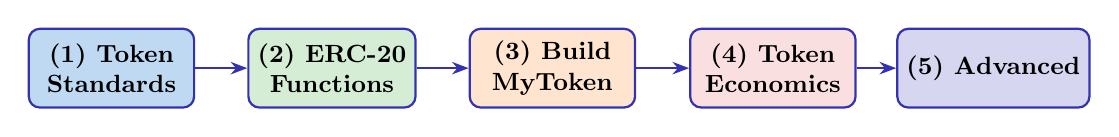
\begin{tikzpicture}[
    procstep/.style={rectangle, rounded corners=4pt, minimum width=2.1cm, minimum height=1.0cm,
      draw=mlpurple, thick, align=center, font=\small\bfseries}
  ]
    \node[procstep, fill=mlblue!25] (b1) at (0,0)    {(1) Token\\Standards};
    \node[procstep, fill=mlgreen!20] (b2) at (2.8,0)  {(2) ERC-20\\Functions};
    \node[procstep, fill=mlorange!20] (b3) at (5.6,0) {(3) Build\\MyToken};
    \node[procstep, fill=mlred!15]   (b4) at (8.4,0)  {(4) Token\\Economics};
    \node[procstep, fill=mlpurple!20](b5) at (11.2,0) {(5) Advanced};
    \draw[-{Stealth[length=6pt]}, thick, mlpurple] (b1.east) -- (b2.west);
    \draw[-{Stealth[length=6pt]}, thick, mlpurple] (b2.east) -- (b3.west);
    \draw[-{Stealth[length=6pt]}, thick, mlpurple] (b3.east) -- (b4.west);
    \draw[-{Stealth[length=6pt]}, thick, mlpurple] (b4.east) -- (b5.west);
  \end{tikzpicture}

  \vspace{4mm}
  \begin{columns}[T]
    \begin{column}{0.48\textwidth}
      \begin{block}{Learning Objectives}
        \begin{itemize}\setlength\itemsep{1pt}
          \item Understand the ERC-20 standard and its role
          \item Implement all required functions and events
          \item Deploy and verify a custom ERC-20 token
          \item Analyze token economic models quantitatively
          \item Explore advanced patterns: minting, burning, voting
        \end{itemize}
      \end{block}
    \end{column}
    \begin{column}{0.48\textwidth}
      \begin{block}{Prerequisites}
        \begin{itemize}\setlength\itemsep{1pt}
          \item Lessons 1--3: Blockchain, Cryptography, Ethereum
          \item Basic Solidity syntax (variables, functions, mappings)
          \item Familiarity with Remix IDE or Hardhat
          \item Understanding of gas and transaction fees
        \end{itemize}
      \end{block}
    \end{column}
  \end{columns}
  \bottomnote{Duration: 90 minutes | 5 sections | \textasciitilde55 frames | Prerequisite: Lessons 1--3}
\end{frame}

% Frame 3: Table of Contents
\begin{frame}{Table of Contents}
  \tableofcontents
  \bottomnote{Navigate through 5 sections covering token standards to deployment}
\end{frame}

\begin{frame}{Learning Objectives}
By the end of this lecture, you will be able to:
\begin{enumerate}
\item \textbf{Explain} the ERC-20 token standard interface and its role in the Ethereum ecosystem
\item \textbf{Implement} a custom ERC-20 token with mint, burn, and access control features
\item \textbf{Analyze} the approve/transferFrom delegation pattern and its security implications
\item \textbf{Compare} fixed, inflationary, and deflationary token supply models
\item \textbf{Design} a token distribution strategy with vesting schedules
\end{enumerate}
\bottomnote{Bloom's taxonomy levels: Remember $\rightarrow$ Understand $\rightarrow$ Apply $\rightarrow$ Analyze $\rightarrow$ Evaluate $\rightarrow$ Create}
\end{frame}

%% ============================================================
%% SECTION 1: TOKEN STANDARDS
%% ============================================================

\section{Token Standards}

% Frame 4: Section Divider
\begin{frame}{}
  \vfill
  \begin{beamercolorbox}[wd=\textwidth, sep=12pt, center, rounded=true]{palette quaternary}
    \LARGE\textbf{Section 1: Token Standards}\\[6pt]
    \normalsize\textcolor{mllavender2}{What tokens are, why standards matter, and the ERC-20 ecosystem}
  \end{beamercolorbox}
  \vfill
  \bottomnote{Section 1 of 5 | Frames 4--14 | Estimated time: 18 minutes}
\end{frame}

% Frame 5: What is a Token?
\begin{frame}{What is a Token?}
  \begin{columns}[T]
    \begin{column}{0.50\textwidth}
      \begin{block}{Coins vs.\ Tokens}
        \textbf{Native Coins:}
        \begin{itemize}\setlength\itemsep{1pt}
          \item Have their own blockchain (BTC, ETH, SOL)
          \item Maintained by network validators/miners
          \item Required for gas / transaction fees
          \item Cannot be created by anyone
        \end{itemize}
        \vspace{3pt}
        \textbf{Tokens:}
        \begin{itemize}\setlength\itemsep{1pt}
          \item Live on an existing blockchain via smart contracts
          \item Anyone can create in minutes
          \item Inherit chain security and infrastructure
          \item Represent virtually any asset or right
        \end{itemize}
      \end{block}
    \end{column}
    \begin{column}{0.46\textwidth}
      \textbf{Token Use Cases:}\\[3pt]
      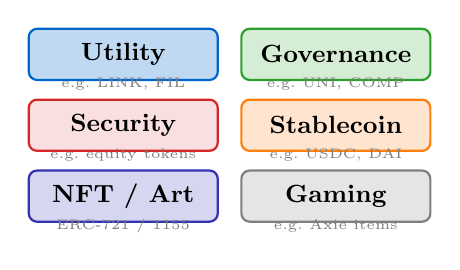
\begin{tikzpicture}
        \tikzset{usecase/.style={rectangle, rounded corners=3pt, minimum width=2.4cm,
            minimum height=0.65cm, draw, thick, text centered, font=\small\bfseries}}
        % Row 1
        \node[usecase, fill=mlblue!25,   draw=mlblue]   (u1) at (0,0)    {Utility};
        \node[usecase, fill=mlgreen!20,  draw=mlgreen]  (u2) at (2.7,0)  {Governance};
        % Row 2
        \node[usecase, fill=mlred!15,    draw=mlred]    (u3) at (0,-0.9) {Security};
        \node[usecase, fill=mlorange!20, draw=mlorange] (u4) at (2.7,-0.9){Stablecoin};
        % Row 3
        \node[usecase, fill=mlpurple!20, draw=mlpurple] (u5) at (0,-1.8) {NFT / Art};
        \node[usecase, fill=mlgray!20,   draw=mlgray]   (u6) at (2.7,-1.8){Gaming};
        % Small example labels
        \node[font=\tiny, text=mlgray] at (0,-0.38)   {e.g.\ LINK, FIL};
        \node[font=\tiny, text=mlgray] at (2.7,-0.38) {e.g.\ UNI, COMP};
        \node[font=\tiny, text=mlgray] at (0,-1.28)   {e.g.\ equity tokens};
        \node[font=\tiny, text=mlgray] at (2.7,-1.28) {e.g.\ USDC, DAI};
        \node[font=\tiny, text=mlgray] at (0,-2.18)   {ERC-721 / 1155};
        \node[font=\tiny, text=mlgray] at (2.7,-2.18) {e.g.\ Axie items};
      \end{tikzpicture}
    \end{column}
  \end{columns}
  \bottomnote{Over 500,000 tokens exist on Ethereum alone, demonstrating the power of token standards}
\end{frame}

% Frame 6: Tokens vs Coins Visual
\begin{frame}{Tokens vs.\ Coins: The Architecture}
  \begin{center}
  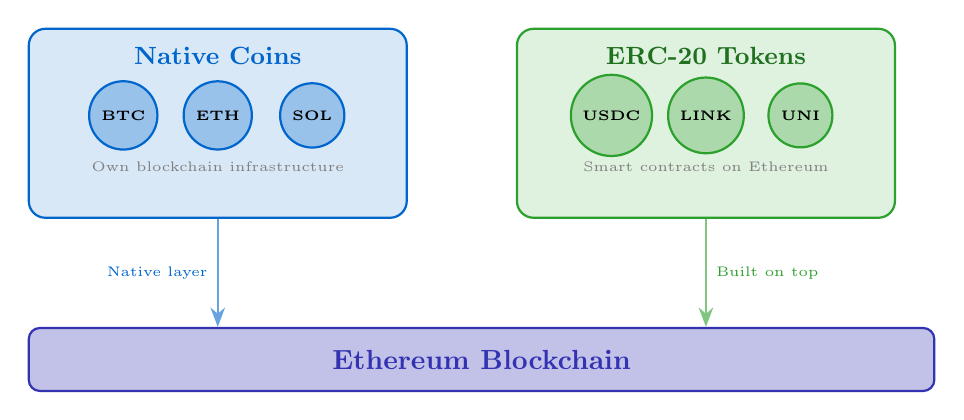
\begin{tikzpicture}[font=\small]
    % Ethereum bar at bottom
    \node[rectangle, rounded corners=4pt, minimum width=11.5cm, minimum height=0.8cm,
          fill=mlpurple!30, draw=mlpurple, thick, text=mlpurple, font=\bfseries]
          (eth) at (5.75,-3.0) {Ethereum Blockchain};

    % Native Coins box — left
    \node[rectangle, rounded corners=6pt, minimum width=4.8cm, minimum height=2.4cm,
          fill=mlblue!15, draw=mlblue, thick]
          (coins) at (2.4,0) {};
    \node[font=\bfseries\small, text=mlblue] at (2.4, 0.85) {Native Coins};
    \node[circle, fill=mlblue!40, draw=mlblue, thick, minimum size=0.75cm,
          font=\bfseries\tiny] (btc) at (1.2, 0.1) {BTC};
    \node[circle, fill=mlblue!40, draw=mlblue, thick, minimum size=0.75cm,
          font=\bfseries\tiny] (eth2) at (2.4, 0.1) {ETH};
    \node[circle, fill=mlblue!40, draw=mlblue, thick, minimum size=0.75cm,
          font=\bfseries\tiny] (sol) at (3.6, 0.1) {SOL};
    \node[font=\tiny, text=mlgray] at (2.4,-0.55) {Own blockchain infrastructure};

    % ERC-20 Tokens box — right
    \node[rectangle, rounded corners=6pt, minimum width=4.8cm, minimum height=2.4cm,
          fill=mlgreen!15, draw=mlgreen, thick]
          (tokens) at (8.6,0) {};
    \node[font=\bfseries\small, text=mlgreen!70!black] at (8.6, 0.85) {ERC-20 Tokens};
    \node[circle, fill=mlgreen!40, draw=mlgreen, thick, minimum size=0.75cm,
          font=\bfseries\tiny] (usdc) at (7.4, 0.1) {USDC};
    \node[circle, fill=mlgreen!40, draw=mlgreen, thick, minimum size=0.75cm,
          font=\bfseries\tiny] (link) at (8.6, 0.1) {LINK};
    \node[circle, fill=mlgreen!40, draw=mlgreen, thick, minimum size=0.75cm,
          font=\bfseries\tiny] (uni) at (9.8, 0.1) {UNI};
    \node[font=\tiny, text=mlgray] at (8.6,-0.55) {Smart contracts on Ethereum};

    % Arrows
    \draw[-{Stealth[length=7pt]}, thick, mlblue!60]
      (coins.south) -- node[left, font=\tiny, text=mlblue]{Native layer} (eth.north -| coins.south);
    \draw[-{Stealth[length=7pt]}, thick, mlgreen!60]
      (tokens.south) -- node[right, font=\tiny, text=mlgreen]{Built on top} (eth.north -| tokens.south);
  \end{tikzpicture}
  \end{center}
  \bottomnote{Coins have their own blockchain; tokens are smart contracts on an existing chain}
\end{frame}

% Frame 7: Why Standards Matter
\begin{frame}{Why Standards Matter}
  \begin{columns}[T]
    \begin{column}{0.46\textwidth}
      \begin{block}{Without Standards}
        \begin{itemize}\setlength\itemsep{2pt}
          \item \textcolor{mlred}{$\times$} Each token has a custom interface
          \item \textcolor{mlred}{$\times$} Wallets must update code for every new token
          \item \textcolor{mlred}{$\times$} No interoperability between protocols
          \item \textcolor{mlred}{$\times$} DEXs cannot swap arbitrary tokens
          \item \textcolor{mlred}{$\times$} Developers duplicate security audits repeatedly
          \item \textcolor{mlred}{$\times$} Massive coordination overhead
        \end{itemize}
      \end{block}
    \end{column}
    \begin{column}{0.46\textwidth}
      \begin{block}{With Standards (ERC-20)}
        \begin{itemize}\setlength\itemsep{2pt}
          \item \textcolor{mlgreen}{$\checkmark$} Universal interface for all tokens
          \item \textcolor{mlgreen}{$\checkmark$} Any wallet works instantly with new tokens
          \item \textcolor{mlgreen}{$\checkmark$} Instant composability in DeFi
          \item \textcolor{mlgreen}{$\checkmark$} DEXs swap any pair automatically
          \item \textcolor{mlgreen}{$\checkmark$} Shared security through OpenZeppelin
          \item \textcolor{mlgreen}{$\checkmark$} Network effects multiply value
        \end{itemize}
      \end{block}
    \end{column}
  \end{columns}
  \vspace{4pt}
  \begin{block}{Analogy: Gift Cards}
    \small
    Imagine if every shop had a different gift card shape, size, and reader.
    ERC-20 is like a universal gift card standard: \textbf{one reader, infinite issuers.}
    Uniswap, Aave, MetaMask --- all read the same interface regardless of which team
    deployed the token.
  \end{block}
  \bottomnote{ERC = Ethereum Request for Comments | ERC-20 proposed 2015 by Fabian Vogelsteller}
\end{frame}

% Frame 8: Standardization Timeline
\begin{frame}{Token Standardization Timeline}
  \begin{center}
  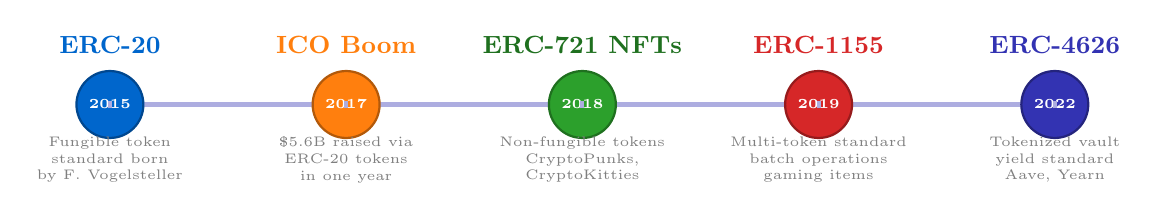
\begin{tikzpicture}[font=\small]
    % Main timeline line
    \draw[line width=2pt, mlpurple!40] (0,0) -- (12,0);

    % Nodes: positions 0, 3, 6, 9, 12
    % 2015: ERC-20
    \node[circle, fill=mlblue, draw=mlblue!70!black, thick,
          minimum size=0.85cm, font=\bfseries\tiny, text=white] (n1) at (0,0) {2015};
    \node[font=\small\bfseries, text=mlblue] at (0, 0.75) {ERC-20};
    \node[font=\tiny, text=mlgray, align=center] at (0,-0.7)
      {Fungible token\\standard born\\by F.\ Vogelsteller};

    % 2017: ICO Boom
    \node[circle, fill=mlorange, draw=mlorange!70!black, thick,
          minimum size=0.85cm, font=\bfseries\tiny, text=white] (n2) at (3,0) {2017};
    \node[font=\small\bfseries, text=mlorange] at (3, 0.75) {ICO Boom};
    \node[font=\tiny, text=mlgray, align=center] at (3,-0.7)
      {\$5.6B raised via\\ERC-20 tokens\\in one year};

    % 2018: ERC-721
    \node[circle, fill=mlgreen, draw=mlgreen!70!black, thick,
          minimum size=0.85cm, font=\bfseries\tiny, text=white] (n3) at (6,0) {2018};
    \node[font=\small\bfseries, text=mlgreen!70!black] at (6, 0.75) {ERC-721 NFTs};
    \node[font=\tiny, text=mlgray, align=center] at (6,-0.7)
      {Non-fungible tokens\\CryptoPunks,\\CryptoKitties};

    % 2019: ERC-1155
    \node[circle, fill=mlred, draw=mlred!70!black, thick,
          minimum size=0.85cm, font=\bfseries\tiny, text=white] (n4) at (9,0) {2019};
    \node[font=\small\bfseries, text=mlred] at (9, 0.75) {ERC-1155};
    \node[font=\tiny, text=mlgray, align=center] at (9,-0.7)
      {Multi-token standard\\batch operations\\gaming items};

    % 2022: ERC-4626
    \node[circle, fill=mlpurple, draw=mlpurple!70!black, thick,
          minimum size=0.85cm, font=\bfseries\tiny, text=white] (n5) at (12,0) {2022};
    \node[font=\small\bfseries, text=mlpurple] at (12, 0.75) {ERC-4626};
    \node[font=\tiny, text=mlgray, align=center] at (12,-0.7)
      {Tokenized vault\\yield standard\\Aave, Yearn};

    % Connecting ticks
    \foreach \x in {0,3,6,9,12}{
      \draw[mlpurple!40, line width=1.5pt] (\x,-0.05) -- (\x,0.05);
    }
  \end{tikzpicture}
  \end{center}
  \bottomnote{Token standards evolved to meet increasingly complex DeFi and NFT use cases}
\end{frame}

% Frame 9: ERC-20 Fungible Token Standard
\begin{frame}{ERC-20: The Fungible Token Standard}
  \begin{columns}[T]
    \begin{column}{0.50\textwidth}
      \begin{block}{Definition}
        \small
        A \textbf{fungible token} standard means every unit is \emph{identical}
        and interchangeable. 1 USDC always equals 1 USDC regardless of which
        address holds it --- unlike an NFT where each token is unique.
      \end{block}
      \vspace{4pt}
      \begin{block}{Fungibility Principle}
        \small
        \begin{itemize}\setlength\itemsep{2pt}
          \item \textbf{Identical:} token\#1 = token\#2 in value
          \item \textbf{Divisible:} up to 18 decimal places ($10^{18}$ units)
          \item \textbf{Interchangeable:} swap any unit freely
          \item \textbf{Uniform:} same rights for all holders
        \end{itemize}
        \vspace{3pt}
        Like currency: \$5 bill A = \$5 bill B, unlike CryptoPunk \#1 $\neq$ \#2
      \end{block}
    \end{column}
    \begin{column}{0.46\textwidth}
      \begin{block}{Required Interface (EIP-20)}
        \textbf{6 Functions:}
        \begin{itemize}\setlength\itemsep{1pt}
          \item {\small\ttfamily totalSupply()} \textcolor{mlgray}{-- total tokens minted}
          \item {\small\ttfamily balanceOf(addr)} \textcolor{mlgray}{-- balance query}
          \item {\small\ttfamily transfer(to, amt)} \textcolor{mlgray}{-- direct send}
          \item {\small\ttfamily approve(spender, amt)} \textcolor{mlgray}{-- grant allowance}
          \item {\small\ttfamily allowance(owner, spender)} \textcolor{mlgray}{-- query limit}
          \item {\small\ttfamily transferFrom(from, to, amt)} \textcolor{mlgray}{-- delegated}
        \end{itemize}
        \vspace{3pt}
        \textbf{2 Events:}
        \begin{itemize}\setlength\itemsep{1pt}
          \item {\small\ttfamily Transfer(from, to, value)}
          \item {\small\ttfamily Approval(owner, spender, value)}
        \end{itemize}
      \end{block}
    \end{column}
  \end{columns}
  \bottomnote{Any contract implementing these 6 functions and 2 events is ERC-20 compliant}
\end{frame}

% Frame 10: ERC-20 Interface Architecture
\begin{frame}{ERC-20 Interface Architecture}
  \begin{center}
  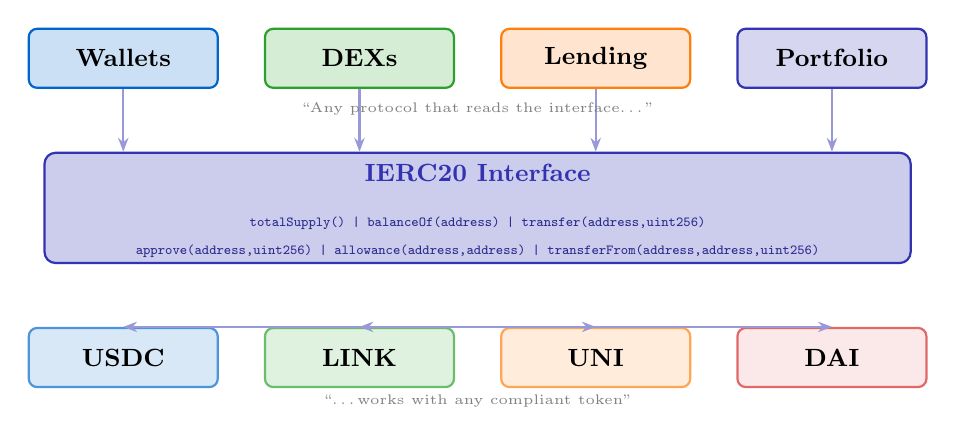
\begin{tikzpicture}[font=\small, node distance=0.6cm]
    % Top row: consumers
    \tikzset{consumer/.style={rectangle, rounded corners=3pt, minimum width=2.4cm,
      minimum height=0.75cm, draw, thick, text centered, font=\small\bfseries}}
    \tikzset{implbox/.style={rectangle, rounded corners=3pt, minimum width=2.4cm,
      minimum height=0.75cm, draw, thick, text centered, font=\small\bfseries}}

    \node[consumer, fill=mlblue!20,    draw=mlblue]   (w1) at (0,2.8)    {Wallets};
    \node[consumer, fill=mlgreen!20,   draw=mlgreen]  (w2) at (3.0,2.8)  {DEXs};
    \node[consumer, fill=mlorange!20,  draw=mlorange] (w3) at (6.0,2.8)  {Lending};
    \node[consumer, fill=mlpurple!20,  draw=mlpurple] (w4) at (9.0,2.8)  {Portfolio};

    % Middle: Interface bar
    \node[rectangle, minimum width=11.0cm, minimum height=1.4cm,
          fill=mlpurple!25, draw=mlpurple, thick, rounded corners=4pt] (iface) at (4.5,0.9) {};
    \node[font=\bfseries\small, text=mlpurple] at (4.5, 1.35) {IERC20 Interface};
    \node[font=\ttfamily\tiny, text=mlpurple!80!black, align=center] at (4.5, 0.7)
      {totalSupply() | balanceOf(address) | transfer(address,uint256)};
    \node[font=\ttfamily\tiny, text=mlpurple!80!black, align=center] at (4.5, 0.35)
      {approve(address,uint256) | allowance(address,address) | transferFrom(address,address,uint256)};

    % Bottom row: implementations
    \node[implbox, fill=mlblue!15,    draw=mlblue!70]  (t1) at (0,-1.0)  {USDC};
    \node[implbox, fill=mlgreen!15,   draw=mlgreen!70] (t2) at (3.0,-1.0) {LINK};
    \node[implbox, fill=mlorange!15,  draw=mlorange!70](t3) at (6.0,-1.0) {UNI};
    \node[implbox, fill=mlred!10,     draw=mlred!70]   (t4) at (9.0,-1.0) {DAI};

    % Arrows top -> interface
    \foreach \w in {w1, w2, w3, w4}{
      \draw[-{Stealth[length=5pt]}, thick, mlpurple!50] (\w.south) -- (\w.south |- iface.north);
    }
    % Arrows interface -> tokens
    \foreach \t in {t1, t2, t3, t4}{
      \draw[-{Stealth[length=5pt]}, thick, mlpurple!50] (iface.south |- \t.north) -- (\t.north);
    }

    % Labels
    \node[font=\tiny, text=mlgray] at (4.5, 2.15) {``Any protocol that reads the interface\ldots''};
    \node[font=\tiny, text=mlgray] at (4.5,-1.55) {``\ldots works with any compliant token''};
  \end{tikzpicture}
  \end{center}
  \bottomnote{The interface pattern enables any new wallet to instantly support any new token}
\end{frame}

% Frame 11: ERC-20 Function Categories
\begin{frame}{ERC-20 Function Categories}
  \begin{center}
  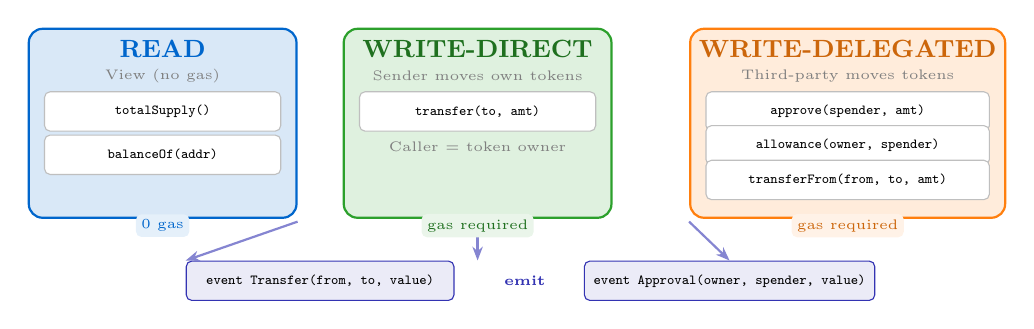
\begin{tikzpicture}[font=\small]
    \tikzset{catbox/.style={rectangle, rounded corners=5pt, minimum width=3.4cm,
      minimum height=2.4cm, draw, thick}}
    \tikzset{fnbox/.style={rectangle, rounded corners=2pt, minimum width=3.0cm,
      minimum height=0.5cm, draw=mlgray!50, fill=white, font=\ttfamily\tiny, text centered}}
    \tikzset{evtbox/.style={rectangle, rounded corners=2pt, minimum width=2.6cm,
      minimum height=0.5cm, draw=mlgray!50, fill=white, font=\ttfamily\tiny, text centered}}

    % READ box
    \node[catbox, fill=mlblue!15, draw=mlblue] (read) at (0,0) {};
    \node[font=\bfseries\small, text=mlblue] at (0, 0.95) {READ};
    \node[font=\tiny, text=mlgray] at (0, 0.60) {View (no gas)};
    \node[fnbox] at (0, 0.15) {\texttt{totalSupply()}};
    \node[fnbox] at (0,-0.40) {\texttt{balanceOf(addr)}};

    % WRITE-DIRECT box
    \node[catbox, fill=mlgreen!15, draw=mlgreen] (direct) at (4.0,0) {};
    \node[font=\bfseries\small, text=mlgreen!70!black] at (4.0, 0.95) {WRITE-DIRECT};
    \node[font=\tiny, text=mlgray] at (4.0, 0.60) {Sender moves own tokens};
    \node[fnbox] at (4.0, 0.15) {\texttt{transfer(to, amt)}};
    \node[font=\tiny, text=mlgray] at (4.0,-0.30) {Caller = token owner};

    % WRITE-DELEGATED box
    \node[catbox, fill=mlorange!15, draw=mlorange, minimum width=4.0cm] (deleg) at (8.7,0) {};
    \node[font=\bfseries\small, text=mlorange!80!black] at (8.7, 0.95) {WRITE-DELEGATED};
    \node[font=\tiny, text=mlgray] at (8.7, 0.60) {Third-party moves tokens};
    \node[fnbox, minimum width=3.6cm] at (8.7, 0.15) {\texttt{approve(spender, amt)}};
    \node[fnbox, minimum width=3.6cm] at (8.7,-0.28) {\texttt{allowance(owner, spender)}};
    \node[fnbox, minimum width=3.6cm] at (8.7,-0.72) {\texttt{transferFrom(from, to, amt)}};

    % Events row
    \node[evtbox, fill=mlpurple!10, draw=mlpurple, minimum width=3.4cm] (ev1) at (2.0,-2.0)
      {\textbf{event} Transfer(from, to, value)};
    \node[evtbox, fill=mlpurple!10, draw=mlpurple, minimum width=3.4cm] (ev2) at (7.2,-2.0)
      {\textbf{event} Approval(owner, spender, value)};
    \node[font=\tiny, text=mlpurple] at (4.6,-2.0) {\textbf{emit}};

    % Emit arrows
    \draw[-{Stealth[length=5pt]}, mlpurple!60, thick]
      ([yshift=-1pt]direct.south) -- (ev1.north -| direct.south);
    \draw[-{Stealth[length=5pt]}, mlpurple!60, thick]
      ([yshift=-1pt]deleg.south west) -- (ev2.north);
    \draw[-{Stealth[length=5pt]}, mlpurple!60, thick]
      ([yshift=-1pt]read.south east) -- (ev1.north west);

    % Gas labels
    \node[font=\tiny, text=mlblue, fill=mlblue!10, rounded corners=2pt,
          inner sep=2pt] at (0,-1.3) {0 gas};
    \node[font=\tiny, text=mlgreen!70!black, fill=mlgreen!10, rounded corners=2pt,
          inner sep=2pt] at (4.0,-1.3) {gas required};
    \node[font=\tiny, text=mlorange!80!black, fill=mlorange!10, rounded corners=2pt,
          inner sep=2pt] at (8.7,-1.3) {gas required};
  \end{tikzpicture}
  \end{center}
  \bottomnote{Read functions cost no gas; write functions require a transaction and gas payment}
\end{frame}

% Frame 12: Other Token Standards
\begin{frame}{Other Token Standards on Ethereum}
  \vspace{4pt}
  \begin{center}
  \begin{tabular}{@{}llllp{3.2cm}@{}}
    \toprule
    \rowcolor{mllavender3}
    \textbf{Standard} & \textbf{Type} & \textbf{Key Feature} & \textbf{Year} & \textbf{Example} \\
    \midrule
    \rowcolor{mllavender4}
    \textbf{ERC-20}   & Fungible Token    & Universal balance interface    & 2015 & USDC, LINK, UNI, DAI \\
    \rowcolor{white}
    \textbf{ERC-721}  & Non-Fungible      & Unique ownership per tokenId   & 2018 & CryptoPunks, BAYC \\
    \rowcolor{mllavender4}
    \textbf{ERC-1155} & Multi-Token       & Batch transfer, fungible+NFT   & 2019 & Gaming items, Enjin \\
    \rowcolor{white}
    \textbf{ERC-4626} & Tokenized Vault   & Standardized yield accounting  & 2022 & Aave aTokens, Yearn \\
    \rowcolor{mllavender4}
    \textbf{ERC-2612} & Permit Extension  & Gasless approvals via signature & 2020 & USDC v2, DAI \\
    \bottomrule
  \end{tabular}
  \end{center}
  \vspace{4pt}
  \begin{columns}[T]
    \begin{column}{0.48\textwidth}
      \begin{block}{ERC-20 Remains Dominant}
        \small
        Despite newer standards, ERC-20 holds $>$90\% of DeFi TVL.
        Most newer standards (ERC-4626, ERC-2612) \emph{extend} ERC-20
        rather than replace it.
      \end{block}
    \end{column}
    \begin{column}{0.48\textwidth}
      \begin{block}{Standard Hierarchy}
        \small
        ERC-721 and ERC-1155 are \emph{not} backward compatible with ERC-20.
        A wallet that reads ERC-20 cannot automatically display NFT holdings ---
        separate interface detection required.
      \end{block}
    \end{column}
  \end{columns}
  \bottomnote{This lecture focuses on ERC-20; other standards build on similar patterns}
\end{frame}

% Frame 13: Token Ecosystem Market Map
\begin{frame}{Token Ecosystem Market Map}
  \begin{center}
  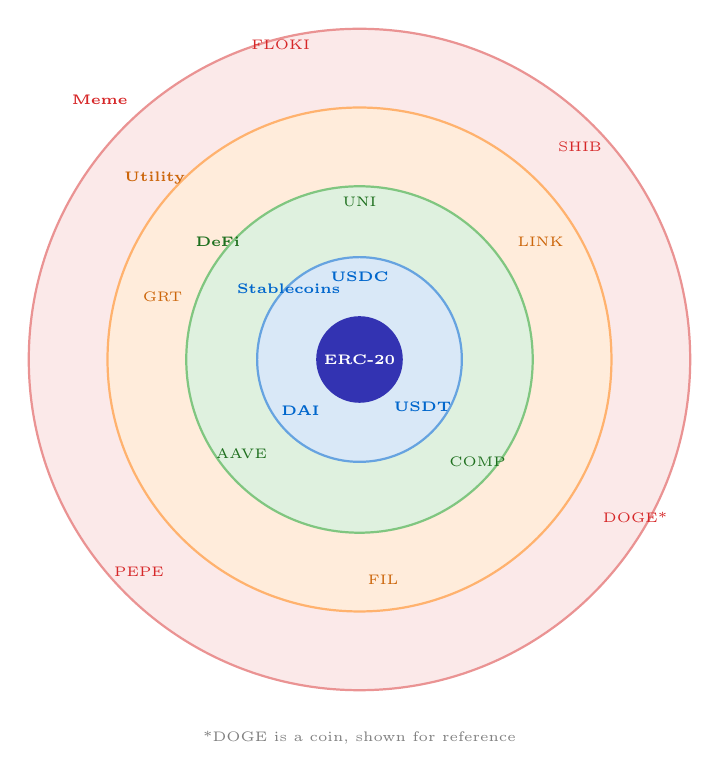
\begin{tikzpicture}[font=\small]
    % Ring 4 (outermost): Meme
    \fill[mlred!10] (0,0) circle (4.2cm);
    \draw[mlred!50, thick] (0,0) circle (4.2cm);

    % Ring 3: Utility
    \fill[mlorange!15] (0,0) circle (3.2cm);
    \draw[mlorange!60, thick] (0,0) circle (3.2cm);

    % Ring 2: DeFi
    \fill[mlgreen!15] (0,0) circle (2.2cm);
    \draw[mlgreen!60, thick] (0,0) circle (2.2cm);

    % Ring 1: Stablecoins
    \fill[mlblue!15] (0,0) circle (1.3cm);
    \draw[mlblue!60, thick] (0,0) circle (1.3cm);

    % Center
    \fill[mlpurple] (0,0) circle (0.55cm);
    \node[font=\bfseries\tiny, text=white] at (0,0) {ERC-20};

    % Ring labels (left side)
    \node[font=\tiny\bfseries, text=mlblue] at (-0.9, 0.9) {Stablecoins};
    \node[font=\tiny\bfseries, text=mlgreen!70!black] at (-1.8, 1.5) {DeFi};
    \node[font=\tiny\bfseries, text=mlorange!80!black] at (-2.6, 2.3) {Utility};
    \node[font=\tiny\bfseries, text=mlred] at (-3.3, 3.3) {Meme};

    % Stablecoin tokens (ring 1, radius ~0.9)
    \node[font=\tiny\bfseries, text=mlblue] at (0, 1.05)    {USDC};
    \node[font=\tiny\bfseries, text=mlblue] at (-0.75,-0.65) {DAI};
    \node[font=\tiny\bfseries, text=mlblue] at (0.80,-0.60)  {USDT};

    % DeFi tokens (ring 2, radius ~1.7)
    \node[font=\tiny, text=mlgreen!70!black] at (0.0, 2.0)   {UNI};
    \node[font=\tiny, text=mlgreen!70!black] at (-1.5,-1.2)  {AAVE};
    \node[font=\tiny, text=mlgreen!70!black] at (1.5,-1.3)   {COMP};

    % Utility tokens (ring 3, radius ~2.7)
    \node[font=\tiny, text=mlorange!80!black] at (2.3, 1.5)  {LINK};
    \node[font=\tiny, text=mlorange!80!black] at (-2.5, 0.8) {GRT};
    \node[font=\tiny, text=mlorange!80!black] at (0.3,-2.8)  {FIL};

    % Meme tokens (ring 4, radius ~3.7)
    \node[font=\tiny, text=mlred] at (2.8, 2.7)   {SHIB};
    \node[font=\tiny, text=mlred] at (-2.8,-2.7)  {PEPE};
    \node[font=\tiny, text=mlred] at (-1.0, 4.0)  {FLOKI};
    \node[font=\tiny, text=mlred] at (3.5,-2.0)   {DOGE*};

    \node[font=\tiny, text=mlgray] at (0,-4.8) {*DOGE is a coin, shown for reference};
  \end{tikzpicture}
  \end{center}
  \bottomnote{The token ecosystem spans from serious financial infrastructure to community-driven experiments}
\end{frame}

% Frame 14: Section 1 Summary — Stat Cards
\begin{frame}{Section 1 Summary: Key Numbers}
  \begin{center}
  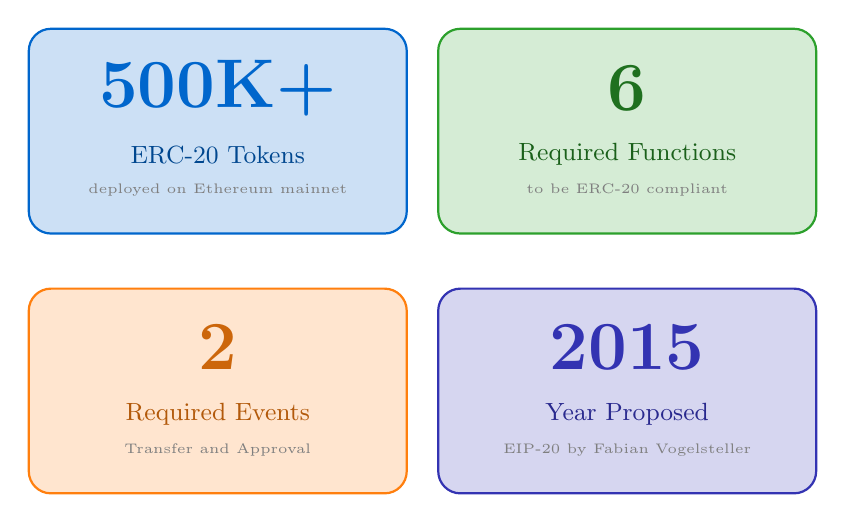
\begin{tikzpicture}[font=\small]
    \tikzset{statcard/.style={rectangle, rounded corners=8pt, minimum width=4.8cm,
      minimum height=2.6cm, draw, thick, text centered}}

    % Card 1: 500K+
    \node[statcard, fill=mlblue!20, draw=mlblue] (c1) at (0,0) {};
    \node[font=\Huge\bfseries, text=mlblue] at (0, 0.55) {500K+};
    \node[font=\small, text=mlblue!70!black] at (0,-0.30) {ERC-20 Tokens};
    \node[font=\tiny, text=mlgray] at (0,-0.75) {deployed on Ethereum mainnet};

    % Card 2: 6
    \node[statcard, fill=mlgreen!20, draw=mlgreen] (c2) at (5.2,0) {};
    \node[font=\Huge\bfseries, text=mlgreen!70!black] at (5.2, 0.55) {6};
    \node[font=\small, text=mlgreen!60!black] at (5.2,-0.30) {Required Functions};
    \node[font=\tiny, text=mlgray] at (5.2,-0.75) {to be ERC-20 compliant};

    % Card 3: 2
    \node[statcard, fill=mlorange!20, draw=mlorange] (c3) at (0,-3.3) {};
    \node[font=\Huge\bfseries, text=mlorange!80!black] at (0,-2.75) {2};
    \node[font=\small, text=mlorange!70!black] at (0,-3.60) {Required Events};
    \node[font=\tiny, text=mlgray] at (0,-4.05) {Transfer and Approval};

    % Card 4: 2015
    \node[statcard, fill=mlpurple!20, draw=mlpurple] (c4) at (5.2,-3.3) {};
    \node[font=\Huge\bfseries, text=mlpurple] at (5.2,-2.75) {2015};
    \node[font=\small, text=mlpurple!80!black] at (5.2,-3.60) {Year Proposed};
    \node[font=\tiny, text=mlgray] at (5.2,-4.05) {EIP-20 by Fabian Vogelsteller};
  \end{tikzpicture}
  \end{center}
  \bottomnote{Token standards are the foundation of the entire DeFi ecosystem}
\end{frame}

% ============================================================
\section{ERC-20 Functions Deep Dive}
% ============================================================

% ----------------------------------------------------------
% Frame 15: Section Divider
% ----------------------------------------------------------
\begin{frame}{~}
  \begin{center}
    \begin{beamercolorbox}[sep=18pt, center, rounded=true, shadow=true]{palette primary}
      \setbeamercolor{palette primary}{bg=mlpurple, fg=white}
      \usebeamercolor[fg]{palette primary}
      {\LARGE\bfseries Section 2: ERC-20 Functions Deep Dive}\\[8pt]
      {\large Understanding each function in detail}
    \end{beamercolorbox}
  \end{center}
\end{frame}

% ----------------------------------------------------------
% Frame 16: totalSupply() and balanceOf()
% ----------------------------------------------------------
\begin{frame}{totalSupply() and balanceOf()}
  \begin{center}
  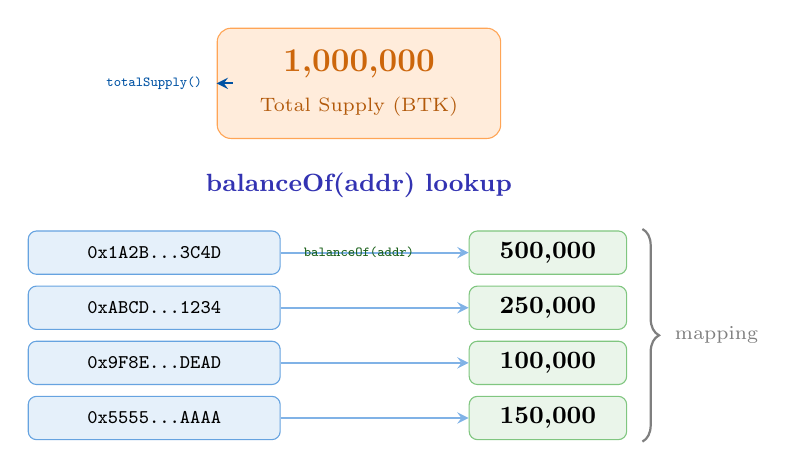
\begin{tikzpicture}[
    addrbox/.style={rectangle, draw=mlblue!60, fill=mlblue!10, rounded corners=3pt,
                    font=\ttfamily\scriptsize, minimum width=3.2cm, minimum height=0.55cm,
                    inner sep=4pt},
    amtbox/.style={rectangle, draw=mlgreen!60, fill=mlgreen!10, rounded corners=3pt,
                   font=\bfseries\small, minimum width=2.0cm, minimum height=0.55cm,
                   inner sep=4pt},
    gaugebox/.style={rectangle, draw=mlorange!70, fill=mlorange!15, rounded corners=5pt,
                     minimum width=3.6cm, minimum height=1.4cm, inner sep=8pt},
    arrlbl/.style={font=\tiny\ttfamily, text=mlpurple},
    >=stealth
  ]
    % --- Gauge (totalSupply) ---
    \node[gaugebox] (gauge) at (0,2.6) {};
    \node[font=\bfseries\large, text=mlorange!80!black] at (0,2.85) {1{,}000{,}000};
    \node[font=\scriptsize, text=mlorange!70!black] at (0,2.30) {Total Supply (BTK)};
    \node[arrlbl, text=mlblue!80!black] at (-2.6, 2.6) {\texttt{totalSupply()}};
    \draw[->, thick, mlblue!80!black] (-1.6,2.6) -- (gauge.west);

    % --- Mapping visualization ---
    \node[font=\small\bfseries, text=mlpurple] at (0,1.3) {balanceOf(addr) lookup};

    % Addresses
    \node[addrbox] (a1) at (-2.6, 0.45) {0x1A2B\ldots{}3C4D};
    \node[addrbox] (a2) at (-2.6,-0.25) {0xABCD\ldots{}1234};
    \node[addrbox] (a3) at (-2.6,-0.95) {0x9F8E\ldots{}DEAD};
    \node[addrbox] (a4) at (-2.6,-1.65) {0x5555\ldots{}AAAA};

    % Balances
    \node[amtbox] (b1) at (2.4, 0.45) {500{,}000};
    \node[amtbox] (b2) at (2.4,-0.25) {250{,}000};
    \node[amtbox] (b3) at (2.4,-0.95) {100{,}000};
    \node[amtbox] (b4) at (2.4,-1.65) {150{,}000};

    % Arrows
    \draw[->, thick, mlblue!50] (a1.east) -- (b1.west);
    \draw[->, thick, mlblue!50] (a2.east) -- (b2.west);
    \draw[->, thick, mlblue!50] (a3.east) -- (b3.west);
    \draw[->, thick, mlblue!50] (a4.east) -- (b4.west);

    % balanceOf label
    \node[arrlbl, text=mlgreen!60!black] at (0, 0.45) {\texttt{balanceOf(addr)}};

    % Bracket around mapping
    \draw[decorate, decoration={brace, amplitude=6pt}, thick, mlgray]
      (3.6,0.75) -- (3.6,-1.95) node[midway, right=8pt, font=\scriptsize, text=mlgray] {mapping};
  \end{tikzpicture}
  \end{center}
  \bottomnote{These are view functions -- they read blockchain state without modifying it}
\end{frame}

% ----------------------------------------------------------
% Frame 17: The Balance Mapping
% ----------------------------------------------------------
\begin{frame}{The Balance Mapping}
  \begin{center}
  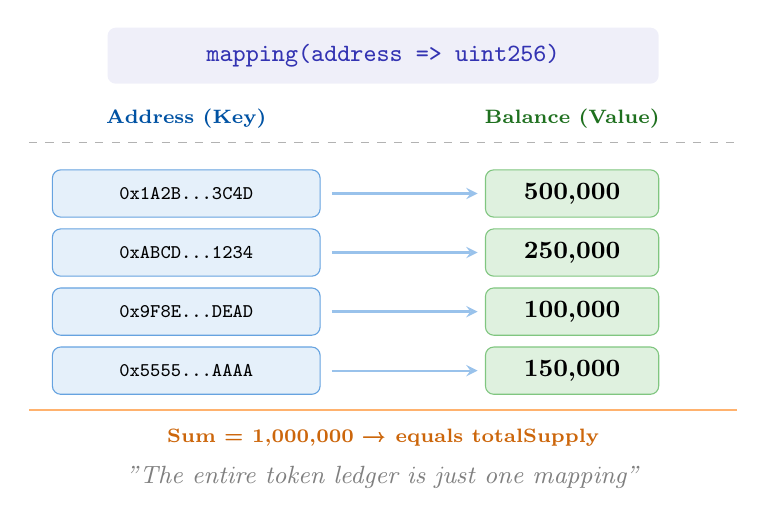
\begin{tikzpicture}[
    kbox/.style={rectangle, draw=mlblue!60, fill=mlblue!10, rounded corners=3pt,
                 font=\ttfamily\scriptsize, minimum width=3.4cm, minimum height=0.6cm, inner sep=4pt},
    vbox/.style={rectangle, draw=mlgreen!60, fill=mlgreen!15, rounded corners=3pt,
                 font=\bfseries\small, minimum width=2.2cm, minimum height=0.6cm, inner sep=4pt},
    >=stealth
  ]
    % Title
    \node[font=\small\ttfamily, text=mlpurple, fill=mlpurple!8, rounded corners=3pt,
          inner sep=6pt, minimum width=7cm] at (0,3.0)
      {mapping(address => uint256)};

    % Key header / Value header
    \node[font=\scriptsize\bfseries, text=mlblue!80!black] at (-2.5, 2.2) {Address (Key)};
    \node[font=\scriptsize\bfseries, text=mlgreen!70!black] at (2.4, 2.2) {Balance (Value)};

    % Separator line
    \draw[mlgray!60, dashed] (-4.5, 1.9) -- (4.5, 1.9);

    % Rows
    \foreach \addr/\bal/\y in {
      {0x1A2B...3C4D}/{500{,}000}/1.25,
      {0xABCD...1234}/{250{,}000}/0.50,
      {0x9F8E...DEAD}/{100{,}000}/-0.25,
      {0x5555...AAAA}/{150{,}000}/-1.00
    }{
      \node[kbox] at (-2.5,\y) {\addr};
      \node[vbox] at (2.4,\y) {\bal};
      \draw[->, thick, mlblue!40] (-0.65,\y) -- (1.2,\y);
    }

    % Sum check
    \draw[mlorange!60, thick] (-4.5,-1.5) -- (4.5,-1.5);
    \node[font=\scriptsize\bfseries, text=mlorange!80!black] at (0,-1.85)
      {Sum = 1{,}000{,}000 \textrightarrow{} equals totalSupply};

    % Caption
    \node[font=\small\itshape, text=mlgray] at (0,-2.35)
      {"The entire token ledger is just one mapping"};
  \end{tikzpicture}
  \end{center}
  \bottomnote{Unlike bank databases, token balances are stored publicly on-chain in a simple mapping}
\end{frame}

% ----------------------------------------------------------
% Frame 18: transfer() Direct Transfer
% ----------------------------------------------------------
\begin{frame}{transfer() -- Direct Transfer}
  \begin{center}
  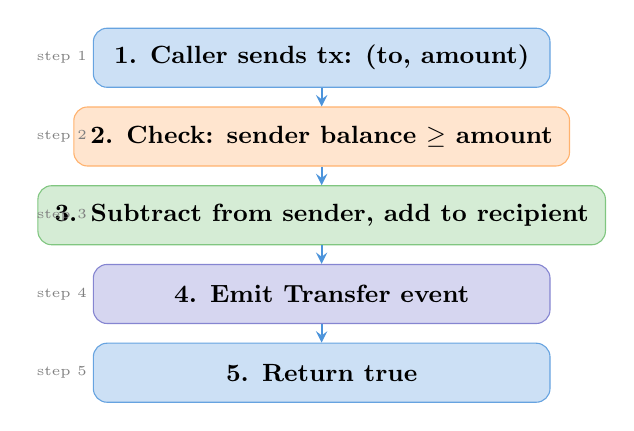
\begin{tikzpicture}[
    stepbox/.style={rectangle, rounded corners=5pt, minimum width=5.8cm,
                    minimum height=0.75cm, inner sep=6pt, font=\small\bfseries},
    >=stealth
  ]
    \node[stepbox, fill=mlblue!20, draw=mlblue!60] (s1) at (0,2.4)
      {1. Caller sends tx: (to, amount)};
    \node[stepbox, fill=mlorange!20, draw=mlorange!60] (s2) at (0,1.4)
      {2. Check: sender balance \(\geq\) amount};
    \node[stepbox, fill=mlgreen!20, draw=mlgreen!60] (s3) at (0,0.4)
      {3. Subtract from sender, add to recipient};
    \node[stepbox, fill=mlpurple!20, draw=mlpurple!60] (s4) at (0,-0.6)
      {4. Emit Transfer event};
    \node[stepbox, fill=mlblue!20, draw=mlblue!60] (s5) at (0,-1.6)
      {5. Return true};

    \draw[->, thick, mlblue!70] (s1.south) -- (s2.north);
    \draw[->, thick, mlblue!70] (s2.south) -- (s3.north);
    \draw[->, thick, mlblue!70] (s3.south) -- (s4.north);
    \draw[->, thick, mlblue!70] (s4.south) -- (s5.north);

    % Step labels
    \foreach \n/\y in {1/2.4, 2/1.4, 3/0.4, 4/-0.6, 5/-1.6}{
      \node[font=\tiny, text=mlgray] at (-3.3, \y) {step \n};
    }
  \end{tikzpicture}
  \end{center}
  \bottomnote{transfer() is the simplest token movement -- you send your own tokens directly}
\end{frame}

% ----------------------------------------------------------
% Frame 19: transfer() Safety Checks
% ----------------------------------------------------------
\begin{frame}{transfer() -- Safety Checks}
  \begin{center}
  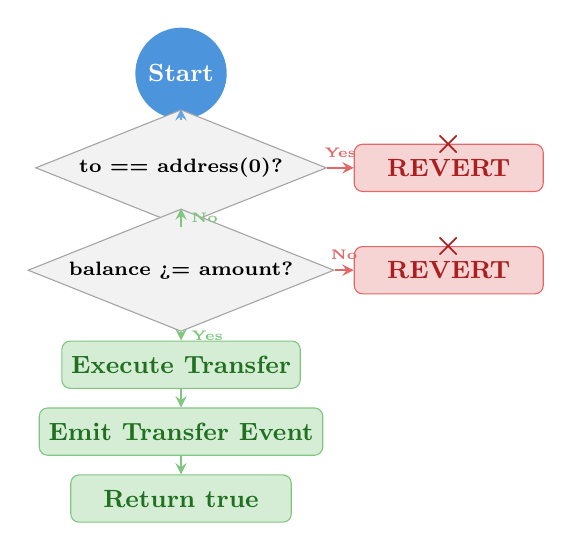
\begin{tikzpicture}[
    startnode/.style={circle, fill=mlblue!70, text=white, font=\bfseries\small,
                      minimum size=0.8cm},
    dnode/.style={diamond, draw=mlgray!70, fill=mlgray!10, font=\scriptsize\bfseries,
                    aspect=2.5, minimum width=3.4cm, minimum height=0.9cm, inner sep=2pt},
    revert/.style={rectangle, rounded corners=3pt, fill=mlred!20, draw=mlred!70,
                   font=\small\bfseries, text=mlred!80!black,
                   minimum width=2.4cm, minimum height=0.6cm},
    proceed/.style={rectangle, rounded corners=3pt, fill=mlgreen!20, draw=mlgreen!60,
                    font=\small\bfseries, text=mlgreen!70!black,
                    minimum width=2.8cm, minimum height=0.6cm},
    >=stealth
  ]
    \node[startnode] (start) at (0,3.2) {Start};
    \node[dnode] (d1) at (0,2.0) {to == address(0)?};
    \node[revert] (r1) at (3.4,2.0) {REVERT};

    \node[dnode] (d2) at (0,0.7) {balance >= amount?};
    \node[revert] (r2) at (3.4,0.7) {REVERT};

    \node[proceed] (exec) at (0,-0.5) {Execute Transfer};
    \node[proceed] (evt) at (0,-1.35) {Emit Transfer Event};
    \node[proceed] (ret) at (0,-2.20) {Return true};

    % Arrows
    \draw[->, thick, mlblue!60] (start) -- (d1);
    \draw[->, thick, mlred!70] (d1.east) -- (r1.west) node[midway, above, font=\tiny\bfseries, text=mlred!70] {Yes};
    \draw[->, thick, mlgreen!60] (d1.south) -- (d2.north) node[midway, right, font=\tiny\bfseries, text=mlgreen!60] {No};
    \draw[->, thick, mlred!70] (d2.east) -- (r2.west) node[midway, above, font=\tiny\bfseries, text=mlred!70] {No};
    \draw[->, thick, mlgreen!60] (d2.south) -- (exec.north) node[midway, right, font=\tiny\bfseries, text=mlgreen!60] {Yes};
    \draw[->, thick, mlgreen!60] (exec) -- (evt);
    \draw[->, thick, mlgreen!60] (evt) -- (ret);

    % Revert cross markers
    \node[font=\large\bfseries, text=mlred!80!black] at (3.4,2.3) {\texttimes};
    \node[font=\large\bfseries, text=mlred!80!black] at (3.4,1.0) {\texttimes};
  \end{tikzpicture}
  \end{center}
  \bottomnote{Every token function must validate inputs before modifying state -- checks-effects-interactions}
\end{frame}

% ----------------------------------------------------------
% Frame 20: approve() and allowance()
% ----------------------------------------------------------
\begin{frame}{approve() and allowance()}
  \begin{center}
  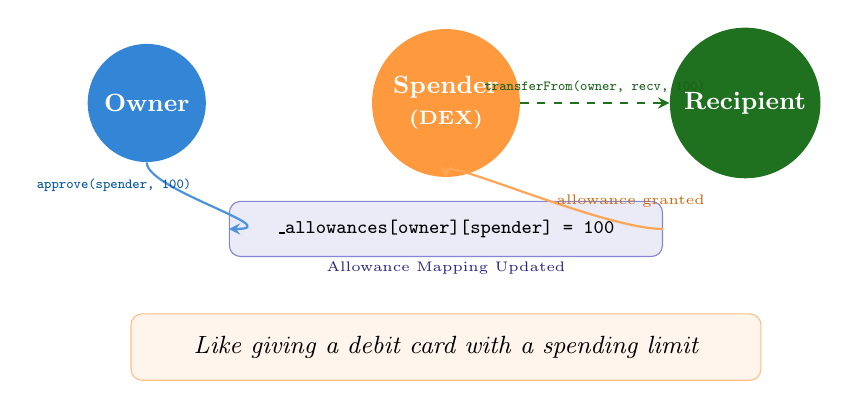
\begin{tikzpicture}[
    actor/.style={circle, minimum size=1.5cm, font=\small\bfseries, text=white,
                  inner sep=4pt, align=center},
    >=stealth
  ]
    % Actors
    \node[actor, fill=mlblue!80] (owner) at (-3.8,1.0) {Owner};
    \node[actor, fill=mlorange!80] (dex) at (0,1.0) {Spender\\{\scriptsize(DEX)}};
    \node[actor, fill=mlgreen!70!black] (recv) at (3.8,1.0) {Recipient};

    % Contract box
    \node[rectangle, draw=mlpurple!60, fill=mlpurple!10, rounded corners=4pt,
          font=\scriptsize\ttfamily, minimum width=5.5cm, minimum height=0.7cm,
          inner sep=5pt] (contract) at (0,-0.6)
      {\_allowances[owner][spender] = 100};
    \node[font=\tiny, text=mlpurple!70!black] at (0,-1.1) {Allowance Mapping Updated};

    % Arrow 1: Owner -> Contract (approve)
    \draw[->, thick, mlblue!70] (owner.south) .. controls (-3.8,-0.1) and (-2.0,-0.6) ..
      (contract.west)
      node[pos=0.45, above left, font=\tiny\ttfamily, text=mlblue!80!black]
        {approve(spender, 100)};

    % Arrow 2: Contract reads allowance for Spender
    \draw[->, thick, mlorange!70] (contract.east) .. controls (2.0,-0.6) and (0,0.3) ..
      (dex.south)
      node[pos=0.45, right, font=\tiny, text=mlorange!80!black]
        {allowance granted};

    % Arrow 3: Spender calls transferFrom later
    \draw[->, thick, mlgreen!70!black, dashed]
      (dex.east) -- (recv.west)
      node[midway, above, font=\tiny\ttfamily, text=mlgreen!60!black]
        {transferFrom(owner, recv, 100)};

    % Analogy box
    \node[rectangle, draw=mlorange!50, fill=mlorange!8, rounded corners=4pt,
          font=\small\itshape, inner sep=8pt, minimum width=8cm] at (0,-2.1)
      {Like giving a debit card with a spending limit};
  \end{tikzpicture}
  \end{center}
  \bottomnote{Approvals are essential for DeFi -- they let smart contracts move tokens on your behalf}
\end{frame}

% ----------------------------------------------------------
% Frame 21: The Allowance Mapping
% ----------------------------------------------------------
\begin{frame}{The Allowance Mapping}
  \begin{center}
  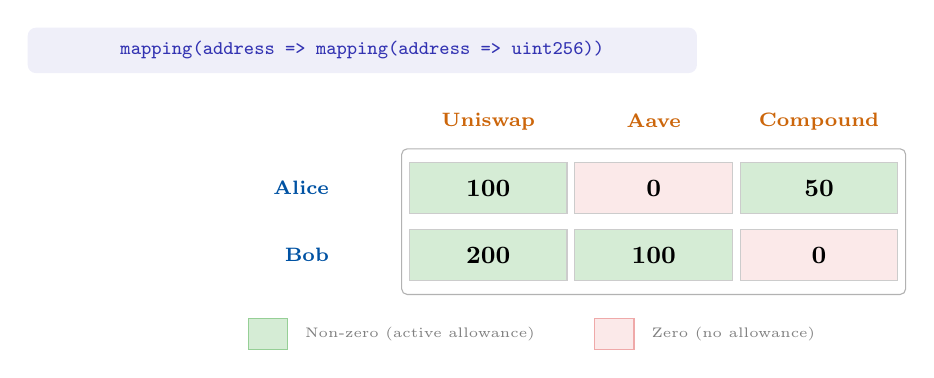
\begin{tikzpicture}[
    cellstyle/.style={rectangle, minimum width=2.0cm, minimum height=0.65cm,
                      inner sep=3pt, font=\small\bfseries, draw=mlgray!40},
    >=stealth
  ]
    % Type annotation
    \node[font=\scriptsize\ttfamily, text=mlpurple, fill=mlpurple!8, rounded corners=3pt,
          inner sep=5pt, minimum width=8.5cm] at (0,3.3)
      {mapping(address => mapping(address => uint256))};

    % Column headers (Spenders)
    \node[font=\scriptsize\bfseries, text=mlorange!80!black] at (1.6,2.4)  {Uniswap};
    \node[font=\scriptsize\bfseries, text=mlorange!80!black] at (3.7,2.4)  {Aave};
    \node[font=\scriptsize\bfseries, text=mlorange!80!black] at (5.8,2.4)  {Compound};

    % Row headers (Owners)
    \node[font=\scriptsize\bfseries, text=mlblue!80!black, anchor=east] at (-0.3,1.55) {Alice};
    \node[font=\scriptsize\bfseries, text=mlblue!80!black, anchor=east] at (-0.3,0.70) {Bob};

    % Cells row Alice
    \node[cellstyle, fill=mlgreen!20] at (1.6,1.55) {100};
    \node[cellstyle, fill=mlred!10]   at (3.7,1.55) {0};
    \node[cellstyle, fill=mlgreen!20] at (5.8,1.55) {50};

    % Cells row Bob
    \node[cellstyle, fill=mlgreen!20] at (1.6,0.70) {200};
    \node[cellstyle, fill=mlgreen!20] at (3.7,0.70) {100};
    \node[cellstyle, fill=mlred!10]   at (5.8,0.70) {0};

    % Legend
    \node[rectangle, fill=mlgreen!20, draw=mlgreen!50, minimum width=0.5cm,
          minimum height=0.4cm] at (-1.2,-0.3) {};
    \node[font=\tiny, anchor=west, text=mlgray] at (-0.85,-0.3) {Non-zero (active allowance)};
    \node[rectangle, fill=mlred!10, draw=mlred!40, minimum width=0.5cm,
          minimum height=0.4cm] at (3.2,-0.3) {};
    \node[font=\tiny, anchor=west, text=mlgray] at (3.55,-0.3) {Zero (no allowance)};

    % Grid border
    \draw[mlgray!60, rounded corners=2pt]
      (0.5,0.2) rectangle (6.9,2.05);
  \end{tikzpicture}
  \end{center}
  \bottomnote{The double mapping allows each owner to set independent allowances for multiple spenders}
\end{frame}

% ----------------------------------------------------------
% Frame 22: transferFrom() Delegated Transfer
% ----------------------------------------------------------
\begin{frame}{transferFrom() -- Delegated Transfer}
  \begin{center}
  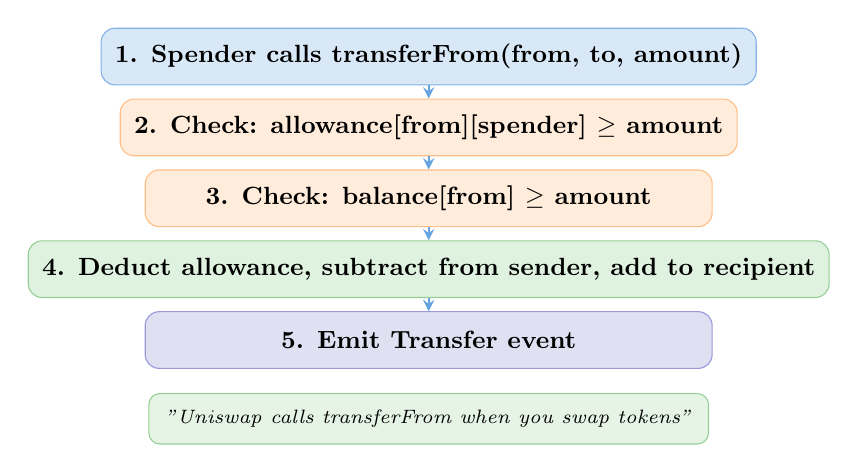
\begin{tikzpicture}[
    stepbox/.style={rectangle, rounded corners=5pt, minimum width=7.2cm,
                    minimum height=0.72cm, inner sep=5pt, font=\small\bfseries},
    callout/.style={rectangle, rounded corners=4pt, fill=mlgreen!12, draw=mlgreen!50,
                    font=\scriptsize\itshape, inner sep=6pt},
    >=stealth
  ]
    \node[stepbox, fill=mlblue!15, draw=mlblue!50] (s1) at (0,2.4)
      {1. Spender calls transferFrom(from, to, amount)};
    \node[stepbox, fill=mlorange!15, draw=mlorange!50] (s2) at (0,1.5)
      {2. Check: allowance[from][spender] \(\geq\) amount};
    \node[stepbox, fill=mlorange!15, draw=mlorange!50] (s3) at (0,0.6)
      {3. Check: balance[from] \(\geq\) amount};
    \node[stepbox, fill=mlgreen!15, draw=mlgreen!50] (s4) at (0,-0.3)
      {4. Deduct allowance, subtract from sender, add to recipient};
    \node[stepbox, fill=mlpurple!15, draw=mlpurple!50] (s5) at (0,-1.2)
      {5. Emit Transfer event};

    \draw[->, thick, mlblue!60] (s1.south) -- (s2.north);
    \draw[->, thick, mlblue!60] (s2.south) -- (s3.north);
    \draw[->, thick, mlblue!60] (s3.south) -- (s4.north);
    \draw[->, thick, mlblue!60] (s4.south) -- (s5.north);

    % Callout box
    \node[callout] at (0,-2.2)
      {"Uniswap calls transferFrom when you swap tokens"};
  \end{tikzpicture}
  \end{center}
  \bottomnote{transferFrom() is the workhorse of DeFi -- every swap, lend, and stake uses it}
\end{frame}

% ----------------------------------------------------------
% Frame 23: Approval Race Condition
% ----------------------------------------------------------
\begin{frame}{Approval Race Condition}
  \begin{center}
  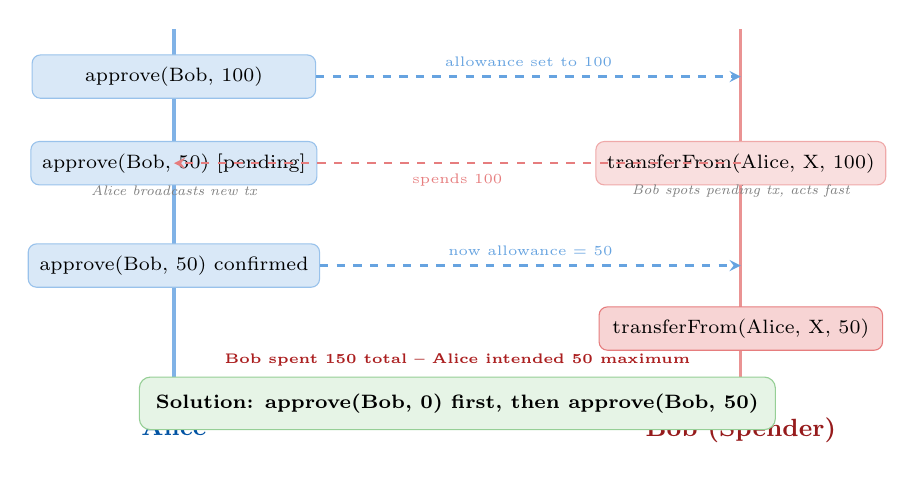
\begin{tikzpicture}[
    event/.style={rectangle, rounded corners=3pt, minimum width=3.6cm,
                  minimum height=0.55cm, inner sep=4pt, font=\scriptsize},
    timeline/.style={->, thick},
    >=stealth
  ]
    % Timelines
    \draw[mlblue!50, very thick] (-3.6,2.0) -- (-3.6,-2.8)
      node[below, font=\small\bfseries, text=mlblue!80!black] {Alice};
    \draw[mlred!50, very thick] (3.6,2.0) -- (3.6,-2.8)
      node[below, font=\small\bfseries, text=mlred!70!black] {Bob (Spender)};

    % Step 1
    \node[event, fill=mlblue!15, draw=mlblue!40] (e1) at (-3.6,1.4)
      {approve(Bob, 100)};
    \draw[->, thick, mlblue!60, dashed] (e1.east) -- (3.6,1.4)
      node[midway, above, font=\tiny] {allowance set to 100};

    % Step 2 (Alice intends to change)
    \node[event, fill=mlblue!15, draw=mlblue!40] (e2) at (-3.6,0.3)
      {approve(Bob, 50) [pending]};
    \node[font=\tiny\itshape, text=mlgray] at (-3.6,-0.05) {Alice broadcasts new tx};

    % Step 3 (Bob front-runs)
    \node[event, fill=mlred!15, draw=mlred!40] (e3) at (3.6,0.3)
      {transferFrom(Alice, X, 100)};
    \node[font=\tiny\itshape, text=mlgray] at (3.6,-0.05) {Bob spots pending tx, acts fast};
    \draw[->, thick, mlred!60, dashed] (3.6,0.3) -- (-3.6,0.3)
      node[midway, below, font=\tiny, text=mlred!60] {spends 100};

    % Step 4 (new approval goes through)
    \node[event, fill=mlblue!15, draw=mlblue!40] (e4) at (-3.6,-1.0)
      {approve(Bob, 50) confirmed};
    \draw[->, thick, mlblue!60, dashed] (e4.east) -- (3.6,-1.0)
      node[midway, above, font=\tiny] {now allowance = 50};

    % Result
    \node[event, fill=mlred!20, draw=mlred!60] (e5) at (3.6,-1.8)
      {transferFrom(Alice, X, 50)};
    \node[font=\tiny\bfseries, text=mlred!80!black] at (0,-2.2)
      {Bob spent 150 total -- Alice intended 50 maximum};

    % Solution
    \node[rectangle, rounded corners=4pt, fill=mlgreen!12, draw=mlgreen!50,
          font=\scriptsize\bfseries, inner sep=6pt, minimum width=8cm] at (0,-2.75)
      {Solution: approve(Bob, 0) first, then approve(Bob, 50)};
  \end{tikzpicture}
  \end{center}
  \bottomnote{The approval race condition is a known ERC-20 issue -- always reset to 0 before changing}
\end{frame}

% ----------------------------------------------------------
% Frame 24: Events -- Transfer and Approval
% ----------------------------------------------------------
\begin{frame}{Events -- Transfer and Approval}
  \begin{center}
  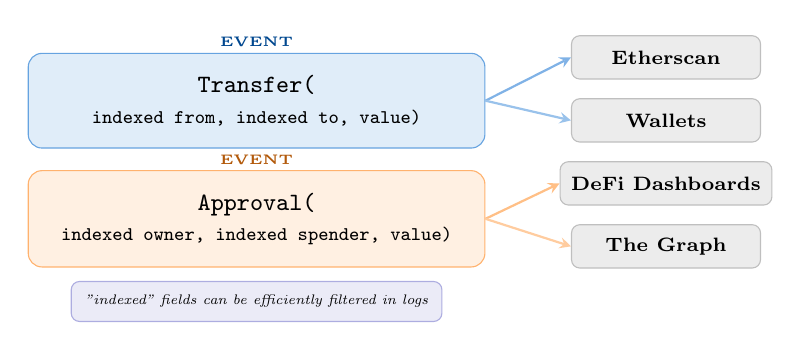
\begin{tikzpicture}[
    eventcard/.style={rectangle, rounded corners=5pt, minimum width=5.8cm,
                      minimum height=1.1cm, inner sep=8pt, font=\small, align=center},
    consumer/.style={rectangle, rounded corners=3pt, fill=mlgray!15, draw=mlgray!50,
                     font=\scriptsize\bfseries, minimum width=2.4cm, minimum height=0.55cm,
                     inner sep=4pt},
    >=stealth
  ]
    % Transfer event card
    \node[eventcard, fill=mlblue!12, draw=mlblue!60] (te) at (-0.2,2.0) {
      \texttt{\bfseries Transfer(}\\
      {\scriptsize\ttfamily \textbf{indexed} from, \textbf{indexed} to, value)}
    };
    \node[font=\tiny\bfseries, text=mlblue!70!black] at (-0.2,2.75) {EVENT};

    % Approval event card
    \node[eventcard, fill=mlorange!12, draw=mlorange!60] (ae) at (-0.2,0.5) {
      \texttt{\bfseries Approval(}\\
      {\scriptsize\ttfamily \textbf{indexed} owner, \textbf{indexed} spender, value)}
    };
    \node[font=\tiny\bfseries, text=mlorange!70!black] at (-0.2,1.25) {EVENT};

    % Consumers
    \node[consumer] (c1) at (5.0, 2.55) {Etherscan};
    \node[consumer] (c2) at (5.0, 1.75) {Wallets};
    \node[consumer] (c3) at (5.0, 0.95) {DeFi Dashboards};
    \node[consumer] (c4) at (5.0, 0.15) {The Graph};

    % Arrows from events to consumers
    \draw[->, thick, mlblue!50]  (te.east) -- (c1.west);
    \draw[->, thick, mlblue!40]  (te.east) -- (c2.west);
    \draw[->, thick, mlorange!50] (ae.east) -- (c3.west);
    \draw[->, thick, mlorange!40] (ae.east) -- (c4.west);

    % "indexed" callout
    \node[rectangle, rounded corners=3pt, fill=mlpurple!10, draw=mlpurple!40,
          font=\tiny\itshape, inner sep=5pt] at (-0.2,-0.55)
      {"indexed" fields can be efficiently filtered in logs};
  \end{tikzpicture}
  \end{center}
  \bottomnote{Events are stored in transaction logs -- cheap storage but cannot be read by other contracts}
\end{frame}

% ----------------------------------------------------------
% Frame 25: Events Power the Ecosystem
% ----------------------------------------------------------
\begin{frame}{Events Power the Ecosystem}
  \begin{center}
  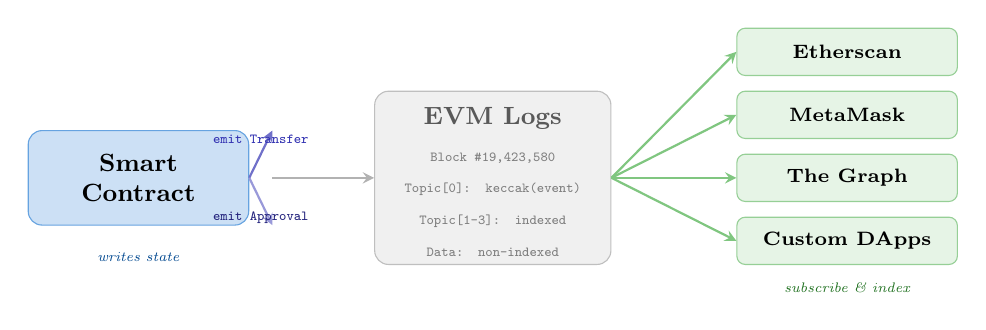
\begin{tikzpicture}[
    mainbox/.style={rectangle, rounded corners=5pt, minimum width=2.8cm,
                    minimum height=1.2cm, inner sep=7pt, font=\small\bfseries, align=center},
    logbox/.style={rectangle, rounded corners=5pt, fill=mlgray!12, draw=mlgray!50,
                   minimum width=3.0cm, minimum height=2.2cm, inner sep=6pt},
    consumer/.style={rectangle, rounded corners=3pt, fill=mlgreen!12, draw=mlgreen!50,
                     font=\scriptsize\bfseries, minimum width=2.8cm, minimum height=0.6cm,
                     inner sep=4pt},
    >=stealth
  ]
    % Smart contract
    \node[mainbox, fill=mlblue!20, draw=mlblue!60] (sc) at (-4.5,0)
      {Smart\\Contract};

    % Emit arrows
    \draw[->, thick, mlpurple!70] (sc.east) -- (-2.8,0.6)
      node[midway, above, font=\tiny\ttfamily, text=mlpurple] {emit Transfer};
    \draw[->, thick, mlpurple!50] (sc.east) -- (-2.8,-0.6)
      node[midway, below, font=\tiny\ttfamily, text=mlpurple!70!black] {emit Approval};

    % EVM Logs box
    \node[logbox] (logs) at (0,0) {};
    \node[font=\small\bfseries, text=mlgray!70!black] at (0,0.75) {EVM Logs};
    \node[font=\tiny\ttfamily, text=mlgray] at (0,0.25) {Block \#19{,}423{,}580};
    \node[font=\tiny\ttfamily, text=mlgray] at (0,-0.15) {Topic[0]: keccak(event)};
    \node[font=\tiny\ttfamily, text=mlgray] at (0,-0.55) {Topic[1-3]: indexed};
    \node[font=\tiny\ttfamily, text=mlgray] at (0,-0.95) {Data: non-indexed};

    % Arrow: contract -> logs
    \draw[->, thick, mlgray!60] (-2.8,0) -- (logs.west);

    % Consumers
    \node[consumer] (p1) at (4.5, 1.6) {Etherscan};
    \node[consumer] (p2) at (4.5, 0.8) {MetaMask};
    \node[consumer] (p3) at (4.5, 0.0) {The Graph};
    \node[consumer] (p4) at (4.5,-0.8) {Custom DApps};

    % Arrows: logs -> consumers
    \draw[->, thick, mlgreen!60] (logs.east) -- (p1.west);
    \draw[->, thick, mlgreen!60] (logs.east) -- (p2.west);
    \draw[->, thick, mlgreen!60] (logs.east) -- (p3.west);
    \draw[->, thick, mlgreen!60] (logs.east) -- (p4.west);

    % Labels
    \node[font=\tiny\itshape, text=mlblue!70!black] at (-4.5,-1.0) {writes state};
    \node[font=\tiny\itshape, text=mlgreen!70!black] at (4.5,-1.4) {subscribe \& index};
  \end{tikzpicture}
  \end{center}
  \bottomnote{Without events, there would be no way to efficiently track token transfers off-chain}
\end{frame}

% ----------------------------------------------------------
% Frame 26: Complete ERC-20 Skeleton  [fragile required!]
% ----------------------------------------------------------
\begin{frame}[fragile]{Complete ERC-20 Skeleton}
\begin{lstlisting}[language=Solidity, basicstyle=\ttfamily\scriptsize,
  keywordstyle=\color{mlblue}\bfseries,
  stringstyle=\color{mlgreen!60!black},
  commentstyle=\color{mlgray}\itshape,
  numbers=left, numberstyle=\tiny\color{mlgray},
  frame=single, rulecolor=\color{mlpurple!40},
  breaklines=true, xleftmargin=12pt]
// SPDX-License-Identifier: MIT
pragma solidity ^0.8.20;

contract BasicERC20 {
    string public name = "BasicToken";
    string public symbol = "BTK";
    uint8 public decimals = 18;
    uint256 public totalSupply;

    mapping(address => uint256) private _balances;
    mapping(address => mapping(address => uint256)) private _allowances;

    event Transfer(address indexed from, address indexed to, uint256 value);
    event Approval(address indexed owner, address indexed spender, uint256 value);

    constructor(uint256 initialSupply) {
        totalSupply = initialSupply * 10**decimals;
        _balances[msg.sender] = totalSupply;
        emit Transfer(address(0), msg.sender, totalSupply);
    }

    function balanceOf(address account) public view returns (uint256) {
        return _balances[account];
    }

    // transfer(), approve(), allowance(), transferFrom() ...
}
\end{lstlisting}
  \bottomnote{This skeleton shows the minimal structure -- production code should use OpenZeppelin}
\end{frame}

% ----------------------------------------------------------
% Frame 27: Function Gas Costs
% ----------------------------------------------------------
\begin{frame}{Function Gas Costs}
  \begin{center}
  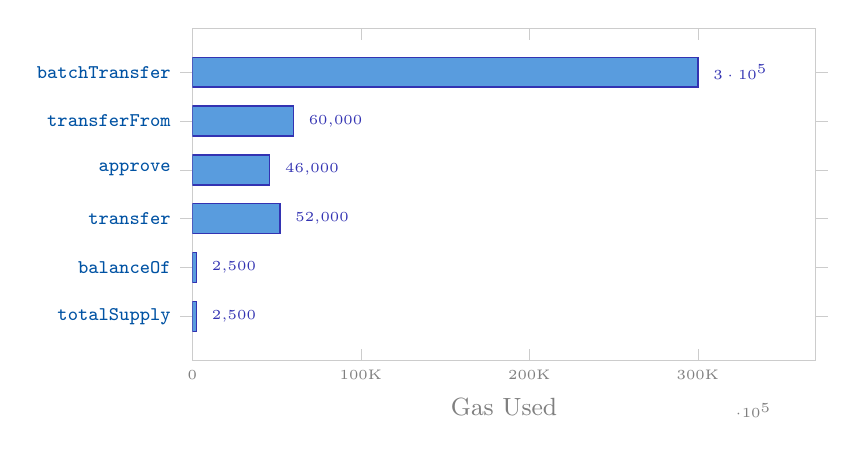
\begin{tikzpicture}
    \begin{axis}[
      xbar,
      width=9.5cm,
      height=5.8cm,
      bar width=0.38cm,
      symbolic y coords={tS,bO,tr,ap,tF,bT},
      yticklabels={totalSupply,balanceOf,transfer,approve,transferFrom,batchTransfer},
      ytick=data,
      xmin=0,
      xmax=370000,
      xlabel={\small Gas Used},
      xlabel style={font=\small, text=mlgray},
      yticklabel style={font=\scriptsize\ttfamily, text=mlblue!80!black},
      xticklabel style={font=\tiny, text=mlgray},
      xtick={0,100000,200000,300000},
      xticklabels={0,100K,200K,300K},
      axis line style={mlgray!40},
      tick style={mlgray!40},
      enlarge y limits=0.18,
      nodes near coords,
      nodes near coords style={font=\tiny\bfseries, text=mlpurple, anchor=west},
      every node near coord/.append style={xshift=2pt},
    ]
      \addplot[fill=mlblue!65, draw=mlpurple, line width=0.5pt] coordinates {
        (2500,tS)
        (2500,bO)
        (52000,tr)
        (46000,ap)
        (60000,tF)
        (300000,bT)
      };
    \end{axis}
  \end{tikzpicture}
  \end{center}
  \bottomnote{View functions are free when called externally; write functions cost real ETH in gas}
\end{frame}

%% ============================================================
%% SECTION 3: BUILD MYTOKEN
%% ============================================================

\section{Build MyToken}

% Frame 28: Section Divider
\begin{frame}{}
  \vfill
  \begin{beamercolorbox}[sep=12pt,center,rounded=true,shadow=true]{palette quaternary}
    \LARGE\bfseries Section 3: Build MyToken\\[6pt]
    \normalsize\mdseries Hands-on: Creating a complete ERC-20 token
  \end{beamercolorbox}
  \vfill
  \bottomnote{We now move from theory to practice -- building a fully functional ERC-20 token from scratch}
\end{frame}

% Frame 29: MyToken Specification
\begin{frame}{MyToken Specification}
  \begin{columns}[T]
    \begin{column}{0.46\textwidth}
      \begin{block}{Token Parameters}
        \vspace{2pt}
        \begin{tabular}{@{}ll@{}}
          \toprule
          \textbf{Property} & \textbf{Value} \\
          \midrule
          Name        & MyToken \\
          Symbol      & MTK \\
          Decimals    & 18 \\
          Max Supply  & 1{,}000{,}000 MTK \\
          Initial Supply & 100{,}000 MTK \\
          \bottomrule
        \end{tabular}
      \end{block}
    \end{column}
    \begin{column}{0.50\textwidth}
      \begin{block}{Features}
        \begin{itemize}\setlength\itemsep{2pt}
          \item \textbf{mint} --- owner-only, capped at MAX\_SUPPLY
          \item \textbf{burn} --- any holder can burn own tokens
          \item \textbf{burnFrom} --- burn with allowance mechanism
          \item \textbf{batchTransfer} --- multiple recipients in one tx
        \end{itemize}
      \end{block}
      \vspace{4pt}
      \begin{block}{Inherits}
        \begin{itemize}\setlength\itemsep{2pt}
          \item OpenZeppelin \texttt{ERC20} --- full standard implementation
          \item OpenZeppelin \texttt{Ownable} --- access control
        \end{itemize}
      \end{block}
    \end{column}
  \end{columns}
  \bottomnote{This design balances simplicity with useful features for learning and experimentation}
\end{frame}

% Frame 30: Design Architecture
\begin{frame}{Design Architecture}
  \begin{center}
  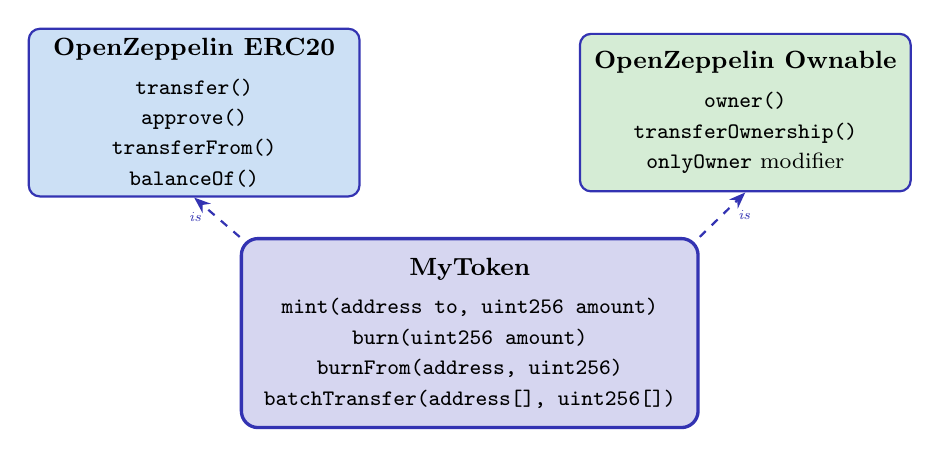
\begin{tikzpicture}[
    parent/.style={rectangle, rounded corners=4pt, minimum width=4.2cm, minimum height=2.0cm,
      draw=mlpurple, thick, align=center, font=\small},
    child/.style={rectangle, rounded corners=6pt, minimum width=5.8cm, minimum height=2.4cm,
      draw=mlpurple, very thick, align=center, font=\small},
    arrow/.style={dashed, -{Stealth[length=6pt]}, thick, mlpurple}
  ]
    % Parent boxes
    \node[parent, fill=mlblue!20] (erc20) at (-3.5, 2.8) {
      \textbf{OpenZeppelin ERC20}\\[3pt]
      {\footnotesize\texttt{transfer()}}\\
      {\footnotesize\texttt{approve()}}\\
      {\footnotesize\texttt{transferFrom()}}\\
      {\footnotesize\texttt{balanceOf()}}
    };
    \node[parent, fill=mlgreen!20] (own) at (3.5, 2.8) {
      \textbf{OpenZeppelin Ownable}\\[3pt]
      {\footnotesize\texttt{owner()}}\\
      {\footnotesize\texttt{transferOwnership()}}\\
      {\footnotesize\texttt{onlyOwner} modifier}
    };
    % Child box
    \node[child, fill=mlpurple!20] (mytoken) at (0, 0) {
      \textbf{MyToken}\\[3pt]
      {\footnotesize\texttt{mint(address to, uint256 amount)}}\\
      {\footnotesize\texttt{burn(uint256 amount)}}\\
      {\footnotesize\texttt{burnFrom(address, uint256)}}\\
      {\footnotesize\texttt{batchTransfer(address[], uint256[])}}
    };
    % Inheritance arrows
    \draw[arrow] (mytoken.north west) -- node[left, font=\tiny\itshape, xshift=-2pt]{\textit{is}} (erc20.south);
    \draw[arrow] (mytoken.north east) -- node[right, font=\tiny\itshape, xshift=2pt]{\textit{is}} (own.south);
  \end{tikzpicture}
  \end{center}
  \bottomnote{Multiple inheritance lets MyToken combine standard token functionality with access control}
\end{frame}

% Frame 31: OpenZeppelin -- Why Not Reinvent?
\begin{frame}{OpenZeppelin -- Why Not Reinvent?}
  \begin{columns}[T]
    \begin{column}{0.44\textwidth}
      \begin{alertblock}{From Scratch}
        \begin{itemize}\setlength\itemsep{3pt}
          \item[\textcolor{mlred}{\textbullet}] 1000+ lines of boilerplate
          \item[\textcolor{mlred}{\textbullet}] Zero security audits
          \item[\textcolor{mlred}{\textbullet}] Error-prone edge cases
          \item[\textcolor{mlred}{\textbullet}] Reinventing known bugs
          \item[\textcolor{mlred}{\textbullet}] Months of hardening needed
        \end{itemize}
      \end{alertblock}
    \end{column}
    \begin{column}{0.44\textwidth}
      \begin{block}{With OpenZeppelin}
        \begin{itemize}\setlength\itemsep{3pt}
          \item[\textcolor{mlgreen}{\textbullet}] \textasciitilde20 lines of custom logic
          \item[\textcolor{mlgreen}{\textbullet}] Battle-tested since 2016
          \item[\textcolor{mlgreen}{\textbullet}] Formally audited code
          \item[\textcolor{mlgreen}{\textbullet}] Community-maintained
          \item[\textcolor{mlgreen}{\textbullet}] Immediate production quality
        \end{itemize}
      \end{block}
    \end{column}
  \end{columns}
  \vspace{6pt}
  \begin{center}
  
\begin{tikzpicture}
    % Shield shape
    \node[draw=mlpurple, very thick, fill=mlpurple!15,
          minimum width=1.4cm, minimum height=1.6cm,
          regular polygon, regular polygon sides=5,
          shape border rotate=0] (shield) at (0,0) {};
    \node[font=\large\bfseries, text=mlpurple] at (shield.center) {\$};
    % Callout bubble
    \node[draw=mlpurple, rounded corners=6pt, fill=mllavender4, align=center,
          font=\small\bfseries, text=mlpurple] at (4.5, 0)
      {$>$\$10B value secured\\by OpenZeppelin contracts};
    \draw[-{Stealth[length=5pt]}, thick, mlpurple] (1.1,0) -- (2.8,0);
  \end{tikzpicture}
  \end{center}
  \bottomnote{OpenZeppelin contracts secure over \$10 billion in value -- never reinvent security-critical code}
\end{frame}

% Frame 32: MyToken.sol -- Complete Contract [CODE]
\begin{frame}[fragile]{MyToken.sol -- The Complete Contract}
\begin{lstlisting}[language=Solidity]
// SPDX-License-Identifier: MIT
pragma solidity ^0.8.20;

import "@openzeppelin/contracts/token/ERC20/ERC20.sol";
import "@openzeppelin/contracts/access/Ownable.sol";

contract MyToken is ERC20, Ownable {
    uint256 public constant MAX_SUPPLY = 1_000_000 * 10**18;

    constructor() ERC20("MyToken", "MTK") Ownable(msg.sender) {
        _mint(msg.sender, 100_000 * 10**18);
    }

    function mint(address to, uint256 amount) public onlyOwner {
        require(totalSupply() + amount <= MAX_SUPPLY, "Exceeds max");
        _mint(to, amount);
    }

    function burn(uint256 amount) public {
        _burn(msg.sender, amount);
    }

    function batchTransfer(address[] calldata to, uint256[] calldata amt)
        external
    {
        require(to.length == amt.length, "Length mismatch");
        for (uint i = 0; i < to.length; i++) {
            _transfer(msg.sender, to[i], amt[i]);
        }
    }
}
\end{lstlisting}
  \bottomnote{Full contract: \textasciitilde30 lines of custom code plus all inherited ERC-20 and Ownable functionality}
\end{frame}

% Frame 33: Constructor Deep Dive
\begin{frame}{Constructor Deep Dive}
  \begin{center}
  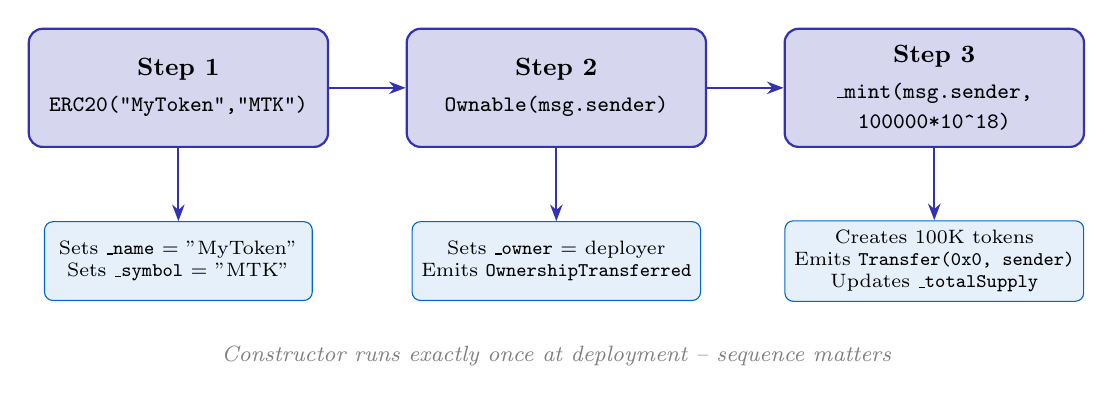
\begin{tikzpicture}[
    stepbox/.style={rectangle, rounded corners=5pt, minimum width=3.8cm, minimum height=1.5cm,
      draw=mlpurple, thick, fill=mllavender4, align=center, font=\small},
    effect/.style={rectangle, rounded corners=3pt, minimum width=3.4cm, minimum height=1.0cm,
      draw=mlblue, fill=mlblue!10, align=center, font=\scriptsize},
    arr/.style={-{Stealth[length=6pt]}, thick, draw=mlpurple}
  ]
    % Step boxes
    \node[stepbox] (s1) at (0, 0) {
      \textbf{Step 1}\\[2pt]
      \texttt{\footnotesize ERC20("MyToken","MTK")}
    };
    \node[stepbox] (s2) at (4.8, 0) {
      \textbf{Step 2}\\[2pt]
      \texttt{\footnotesize Ownable(msg.sender)}
    };
    \node[stepbox] (s3) at (9.6, 0) {
      \textbf{Step 3}\\[2pt]
      \texttt{\footnotesize \_mint(msg.sender,}\\
      \texttt{\footnotesize 100000*10\^{}18)}
    };
    % Effect boxes below
    \node[effect] (e1) at (0, -2.2) {
      Sets \texttt{\_name} = "MyToken"\\
      Sets \texttt{\_symbol} = "MTK"
    };
    \node[effect] (e2) at (4.8, -2.2) {
      Sets \texttt{\_owner} = deployer\\
      Emits \texttt{OwnershipTransferred}
    };
    \node[effect] (e3) at (9.6, -2.2) {
      Creates 100K tokens\\
      Emits \texttt{Transfer(0x0, sender)}\\
      Updates \texttt{\_totalSupply}
    };
    % Arrows
    \draw[arr] (s1) -- (e1);
    \draw[arr] (s2) -- (e2);
    \draw[arr] (s3) -- (e3);
    \draw[arr] (s1.east) -- (s2.west);
    \draw[arr] (s2.east) -- (s3.west);
    % Label
    \node[font=\footnotesize\itshape, text=mlgray] at (4.8, -3.4)
      {Constructor runs exactly once at deployment -- sequence matters};
  \end{tikzpicture}
  \end{center}
  \bottomnote{The constructor runs exactly once during deployment -- it initializes all inherited contracts}
\end{frame}

% Frame 34: The 10^18 Decimals
\begin{frame}{The $10^{18}$ Decimals}
  \begin{center}
  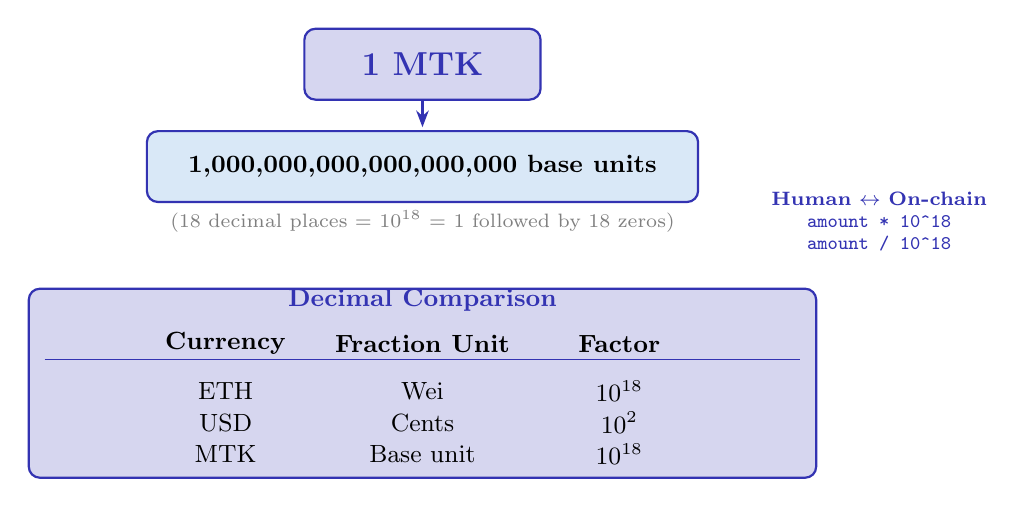
\begin{tikzpicture}[
    box/.style={rectangle, rounded corners=4pt, draw=mlpurple, thick, align=center}
  ]
    % Top label
    \node[box, minimum width=3cm, minimum height=0.9cm, fill=mlpurple!20,
          font=\large\bfseries, text=mlpurple] (human) at (0, 2.5)
      {1 MTK};
    % Equals arrow
    \draw[-{Stealth[length=6pt]}, very thick, mlpurple] (human.south) -- (0, 1.7);
    % Base units
    \node[box, minimum width=7cm, minimum height=0.9cm, fill=mlblue!15,
          font=\small\bfseries] (base) at (0, 1.2)
      {1{,}000{,}000{,}000{,}000{,}000{,}000 base units};
    \node[font=\scriptsize, text=mlgray] at (0, 0.5)
      {(18 decimal places = $10^{18}$ = 1 followed by 18 zeros)};
    % Comparison table
    \begin{scope}[yshift=-10pt]
    \node[box, fill=mllavender4, minimum width=10cm, minimum height=2.4cm] at (0, -1.2) {};
    \node[font=\small\bfseries, text=mlpurple] at (0, -0.15) {Decimal Comparison};
    \node[font=\small] at (-2.5, -0.7) {\textbf{Currency}};
    \node[font=\small] at (0,    -0.7) {\textbf{Fraction Unit}};
    \node[font=\small] at (2.5,  -0.7) {\textbf{Factor}};
    \draw[mlpurple, thin] (-4.8,-0.9) -- (4.8,-0.9);
    \node[font=\small] at (-2.5, -1.3) {ETH};
    \node[font=\small] at (0,    -1.3) {Wei};
    \node[font=\small] at (2.5,  -1.3) {$10^{18}$};
    \node[font=\small] at (-2.5, -1.7) {USD};
    \node[font=\small] at (0,    -1.7) {Cents};
    \node[font=\small] at (2.5,  -1.7) {$10^{2}$};
    \node[font=\small] at (-2.5, -2.1) {MTK};
    \node[font=\small] at (0,    -2.1) {Base unit};
    \node[font=\small] at (2.5,  -2.1) {$10^{18}$};
    \end{scope}
    % Conversion arrow
    \node[font=\scriptsize, text=mlpurple, align=center] at (5.8, 0.5)
      {\textbf{Human} $\leftrightarrow$ \textbf{On-chain}\\
       \texttt{amount * 10\^{}18}\\
       \texttt{amount / 10\^{}18}};
  \end{tikzpicture}
  \end{center}
  \bottomnote{18 decimals allow fractional token amounts down to 0.000000000000000001 MTK}
\end{frame}

% Frame 35: Mint Function
\begin{frame}{Mint Function}
  \begin{center}
  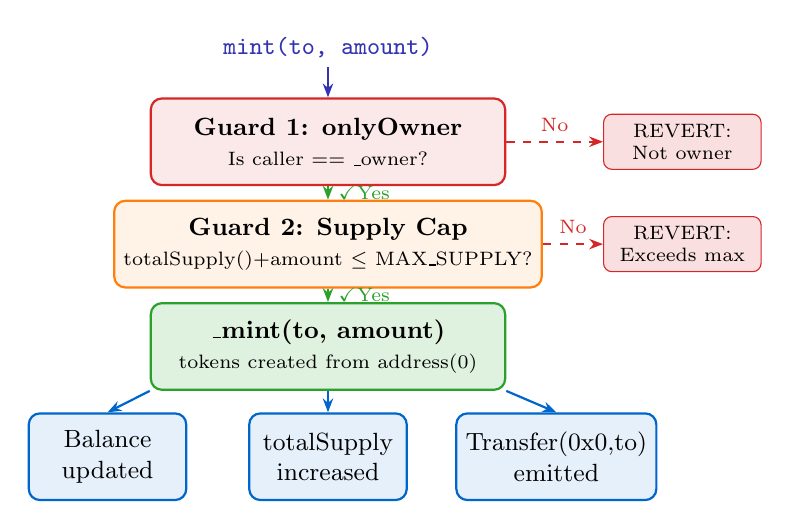
\begin{tikzpicture}[
    guard/.style={rectangle, rounded corners=4pt, minimum width=4.5cm, minimum height=1.1cm,
      draw=mlred, thick, align=center, font=\small},
    action/.style={rectangle, rounded corners=4pt, minimum width=4.5cm, minimum height=1.1cm,
      draw=mlgreen, thick, fill=mlgreen!15, align=center, font=\small},
    revert/.style={rectangle, rounded corners=3pt, minimum width=2.0cm, minimum height=0.7cm,
      draw=mlred, fill=mlred!15, align=center, font=\scriptsize},
    arr/.style={-{Stealth[length=5pt]}, thick},
    revarr/.style={-{Stealth[length=5pt]}, thick, mlred, dashed}
  ]
    % Entry
    \node[font=\small\bfseries, text=mlpurple] (call) at (0, 3.2)
      {\texttt{mint(to, amount)}};
    % Guard 1: onlyOwner
    \node[guard, fill=mlred!10] (g1) at (0, 2.0)
      {\textbf{Guard 1: onlyOwner}\\{\scriptsize Is caller == \_owner?}};
    \node[revert] (r1) at (4.5, 2.0) {REVERT:\\Not owner};
    % Guard 2: supply cap
    \node[guard, fill=mlorange!10, draw=mlorange] (g2) at (0, 0.7)
      {\textbf{Guard 2: Supply Cap}\\{\scriptsize totalSupply()+amount $\leq$ MAX\_SUPPLY?}};
    \node[revert] (r2) at (4.5, 0.7) {REVERT:\\Exceeds max};
    % Action: mint
    \node[action] (a1) at (0, -0.6)
      {\textbf{\_mint(to, amount)}\\{\scriptsize tokens created from address(0)}};
    % Effects
    \node[action, draw=mlblue, fill=mlblue!10, minimum width=2.0cm] (ef1) at (-2.8, -2.0)
      {Balance\\updated};
    \node[action, draw=mlblue, fill=mlblue!10, minimum width=2.0cm] (ef2) at (0, -2.0)
      {totalSupply\\increased};
    \node[action, draw=mlblue, fill=mlblue!10, minimum width=2.5cm] (ef3) at (2.9, -2.0)
      {Transfer(0x0,to)\\emitted};
    % Arrows (green path)
    \draw[arr, mlpurple] (call) -- (g1);
    \draw[arr, mlgreen] (g1.south) -- node[right, font=\scriptsize]{\checkmark Yes} (g2.north);
    \draw[arr, mlgreen] (g2.south) -- node[right, font=\scriptsize]{\checkmark Yes} (a1.north);
    \draw[arr, mlblue] (a1.south west) -- (ef1.north);
    \draw[arr, mlblue] (a1.south) -- (ef2.north);
    \draw[arr, mlblue] (a1.south east) -- (ef3.north);
    % Revert arrows (red path)
    \draw[revarr] (g1.east) -- node[above, font=\scriptsize]{No} (r1.west);
    \draw[revarr] (g2.east) -- node[above, font=\scriptsize]{No} (r2.west);
  \end{tikzpicture}
  \end{center}
  \bottomnote{The MAX\_SUPPLY cap prevents unlimited inflation -- a key tokenomics design decision}
\end{frame}

% Frame 36: Burn Function
\begin{frame}{Burn Function}
  \begin{center}
  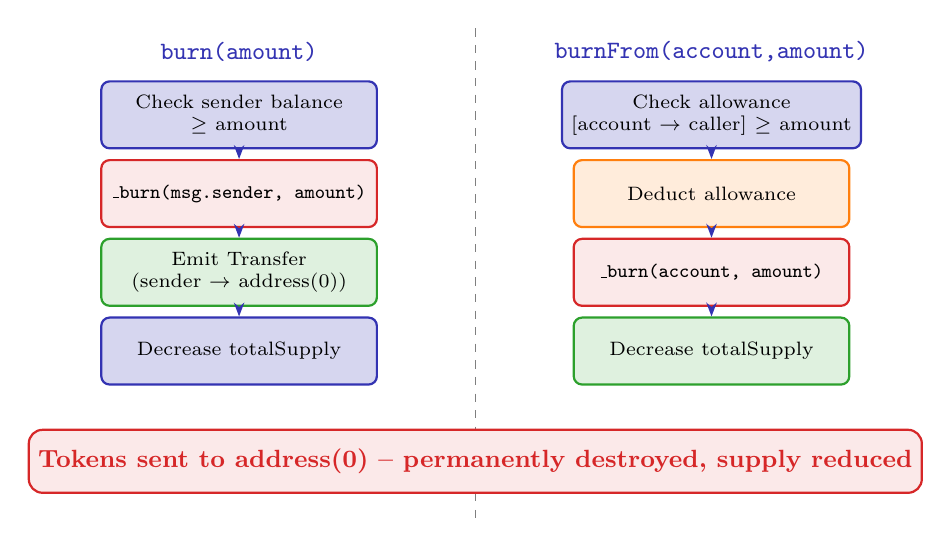
\begin{tikzpicture}[
    stepbox/.style={rectangle, rounded corners=3pt, minimum width=3.5cm, minimum height=0.85cm,
      draw=mlpurple, thick, fill=mllavender4, align=center, font=\scriptsize},
    arr/.style={-{Stealth[length=5pt]}, thick, mlpurple}
  ]
    % Title labels
    \node[font=\small\bfseries, text=mlpurple] at (-3.0, 3.2) {\texttt{burn(amount)}};
    \node[font=\small\bfseries, text=mlpurple] at (3.0, 3.2) {\texttt{burnFrom(account,amount)}};
    \draw[mlgray, dashed] (0, 3.5) -- (0, -2.8);

    % Left path: burn
    \node[stepbox] (l1) at (-3.0, 2.4) {Check sender balance\\$\geq$ amount};
    \node[stepbox, fill=mlred!10, draw=mlred] (l2) at (-3.0, 1.4) {\texttt{\_burn(msg.sender, amount)}};
    \node[stepbox, fill=mlgreen!15, draw=mlgreen] (l3) at (-3.0, 0.4) {Emit Transfer\\(sender $\to$ address(0))};
    \node[stepbox] (l4) at (-3.0, -0.6) {Decrease totalSupply};

    % Right path: burnFrom
    \node[stepbox] (r1) at (3.0, 2.4) {Check allowance\\{}[account $\to$ caller] $\geq$ amount};
    \node[stepbox, fill=mlorange!15, draw=mlorange] (r2) at (3.0, 1.4) {Deduct allowance};
    \node[stepbox, fill=mlred!10, draw=mlred] (r3) at (3.0, 0.4) {\texttt{\_burn(account, amount)}};
    \node[stepbox, fill=mlgreen!15, draw=mlgreen] (r4) at (3.0, -0.6) {Decrease totalSupply};

    % Arrows left
    \draw[arr] (l1) -- (l2);
    \draw[arr] (l2) -- (l3);
    \draw[arr] (l3) -- (l4);

    % Arrows right
    \draw[arr] (r1) -- (r2);
    \draw[arr] (r2) -- (r3);
    \draw[arr] (r3) -- (r4);

    % Bottom note box
    \node[rectangle, rounded corners=5pt, draw=mlred, thick, fill=mlred!10,
          minimum width=9cm, minimum height=0.8cm, align=center, font=\small\bfseries,
          text=mlred] at (0, -2.0)
      {Tokens sent to address(0) -- permanently destroyed, supply reduced};
  \end{tikzpicture}
  \end{center}
  \bottomnote{Burning reduces total supply permanently -- creating scarcity and potential value appreciation}
\end{frame}

% Frame 37: Batch Transfer
\begin{frame}{Batch Transfer -- Gas Efficiency}
  \begin{columns}[T]
    \begin{column}{0.44\textwidth}
      \begin{alertblock}{Individual Transfers (N=10)}
        \begin{center}
        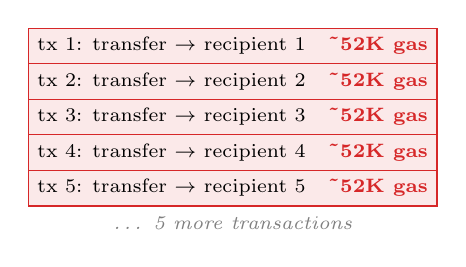
\begin{tikzpicture}[scale=0.82]
          \foreach \i in {1,...,5} {
            \node[rectangle, draw=mlred, fill=mlred!10, minimum width=3.4cm,
                  minimum height=0.45cm, align=center, font=\scriptsize] at (0, -\i*0.55)
              {tx \i: transfer $\to$ recipient \i \quad \textcolor{mlred}{\textbf{\textasciitilde52K gas}}};
          }
          \node[font=\scriptsize\itshape, text=mlgray] at (0, -3.3)
            {\ldots\ 5 more transactions};
        \end{tikzpicture}
        \end{center}
        \vspace{2pt}
        {\small\textbf{Total: 10 $\times$ 52K = 520K gas}}
      \end{alertblock}
    \end{column}
    \begin{column}{0.50\textwidth}
      \begin{block}{Batch Transfer (N=10)}
        \begin{center}
        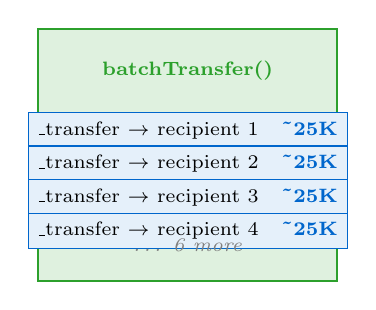
\begin{tikzpicture}[scale=0.82]
          \node[rectangle, draw=mlgreen, thick, fill=mlgreen!15,
                minimum width=3.8cm, minimum height=3.2cm, align=center] (outer) at (0, -1.5) {};
          \node[font=\scriptsize\bfseries, text=mlgreen] at (0, -0.2) {batchTransfer()};
          \foreach \i in {1,...,4} {
            \node[rectangle, draw=mlblue, fill=mlblue!10, minimum width=3.2cm,
                  minimum height=0.38cm, align=center, font=\scriptsize] at (0, -0.6-\i*0.52)
              {\_transfer $\to$ recipient \i \quad \textcolor{mlblue}{\textbf{\textasciitilde25K}}};
          }
          \node[font=\scriptsize\itshape, text=mlgray] at (0, -2.9)
            {\ldots\ 6 more};
        \end{tikzpicture}
        \end{center}
        {\small\textbf{Total: 52K + 10$\times$25K = 302K gas}}
      \end{block}
    \end{column}
  \end{columns}
  \vspace{4pt}
  \begin{center}
    {\small\textbf{Savings:} $520\text{K} - 302\text{K} = 218\text{K}$ gas $\approx$ \textbf{42\% reduction}}
  \end{center}
  \bottomnote{Batch transfers save gas for airdrops and payroll -- one transaction instead of many}
\end{frame}

% Frame 38: Development Workflow
\begin{frame}{Development Workflow}
  \begin{center}
  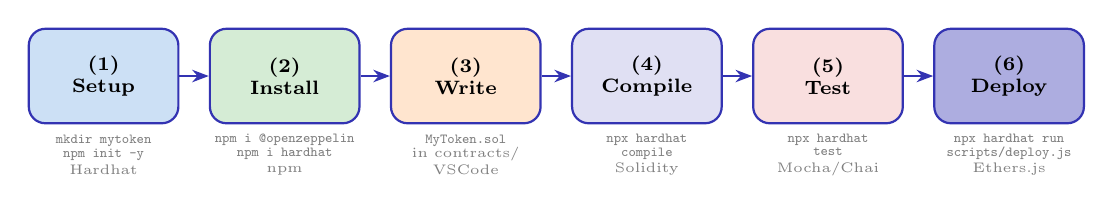
\begin{tikzpicture}[
    wstep/.style={rectangle, rounded corners=6pt, minimum width=1.9cm, minimum height=1.2cm,
      draw=mlpurple, thick, align=center, font=\scriptsize\bfseries},
    tool/.style={font=\tiny, text=mlgray, align=center},
    arr/.style={-{Stealth[length=6pt]}, thick, mlpurple}
  ]
    \node[wstep, fill=mlblue!20]    (s1) at (0.0, 0) {\textbf{(1)}\\Setup};
    \node[wstep, fill=mlgreen!20]   (s2) at (2.3, 0) {\textbf{(2)}\\Install};
    \node[wstep, fill=mlorange!20]  (s3) at (4.6, 0) {\textbf{(3)}\\Write};
    \node[wstep, fill=mlpurple!15]  (s4) at (6.9, 0) {\textbf{(4)}\\Compile};
    \node[wstep, fill=mlred!15]     (s5) at (9.2, 0) {\textbf{(5)}\\Test};
    \node[wstep, fill=mllavender]   (s6) at (11.5, 0){\textbf{(6)}\\Deploy};

    \draw[arr] (s1.east) -- (s2.west);
    \draw[arr] (s2.east) -- (s3.west);
    \draw[arr] (s3.east) -- (s4.west);
    \draw[arr] (s4.east) -- (s5.west);
    \draw[arr] (s5.east) -- (s6.west);

    % Tool labels below
    \node[tool] at (0.0, -1.0) {\texttt{mkdir mytoken}\\[-1pt]\texttt{npm init -y}\\Hardhat};
    \node[tool] at (2.3, -1.0) {\texttt{npm i @openzeppelin}\\[-1pt]\texttt{npm i hardhat}\\npm};
    \node[tool] at (4.6, -1.0) {\texttt{MyToken.sol}\\[-1pt]in contracts/\\VSCode};
    \node[tool] at (6.9, -1.0) {\texttt{npx hardhat}\\[-1pt]\texttt{compile}\\Solidity};
    \node[tool] at (9.2, -1.0) {\texttt{npx hardhat}\\[-1pt]\texttt{test}\\Mocha/Chai};
    \node[tool] at (11.5,-1.0) {\texttt{npx hardhat run}\\[-1pt]\texttt{scripts/deploy.js}\\Ethers.js};
  \end{tikzpicture}
  \end{center}
  \vspace{6pt}
  \begin{block}{Project Structure}
    \centering{\small
    \texttt{mytoken/}\ $\to$\ \texttt{contracts/MyToken.sol}\ |\ \texttt{scripts/deploy.js}\ |\ \texttt{test/MyToken.test.js}\ |\ \texttt{hardhat.config.js}}
  \end{block}
  \bottomnote{Hardhat is the most popular Ethereum development environment -- alternatives include Foundry and Truffle}
\end{frame}

% Frame 39: Deploy Script [CODE]
\begin{frame}[fragile]{Deploy Script}
\begin{lstlisting}[language={},keywords={const,async,function,await,require,console},keywordstyle=\color{solkeyword}\bfseries,commentstyle=\color{solcomment}\ttfamily,stringstyle=\color{solstring}\ttfamily]
const hre = require("hardhat");

async function main() {
    const [deployer] = await hre.ethers.getSigners();
    console.log("Deploying with:", deployer.address);

    const MyToken = await hre.ethers.getContractFactory("MyToken");
    const token = await MyToken.deploy();
    await token.waitForDeployment();

    console.log("MyToken deployed to:", await token.getAddress());
}

main().catch((error) => {
    console.error(error);
    process.exitCode = 1;
});
\end{lstlisting}
  \bottomnote{Run: npx hardhat run scripts/deploy.js --network localhost}
\end{frame}

% Frame 40: Testing Strategy
\begin{frame}{Testing Strategy}
  \begin{center}
  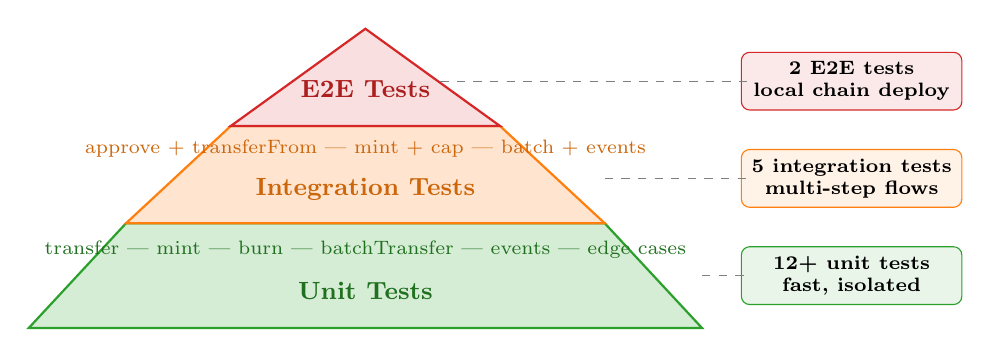
\begin{tikzpicture}[scale=0.95]
    % Test pyramid: E2E at top, Integration middle, Unit at bottom
    % Bottom: Unit tests (wide)
    \fill[mlgreen!20] (-4.5, 0) -- (4.5, 0) -- (3.2, 1.4) -- (-3.2, 1.4) -- cycle;
    \draw[mlgreen, thick] (-4.5, 0) -- (4.5, 0) -- (3.2, 1.4) -- (-3.2, 1.4) -- cycle;
    \node[font=\small\bfseries, text=mlgreen!70!black] at (0, 0.5)
      {Unit Tests};
    \node[font=\scriptsize, text=mlgreen!70!black] at (0, 1.05)
      {transfer | mint | burn | batchTransfer | events | edge cases};

    % Middle: Integration tests
    \fill[mlorange!20] (-3.2, 1.4) -- (3.2, 1.4) -- (1.8, 2.7) -- (-1.8, 2.7) -- cycle;
    \draw[mlorange, thick] (-3.2, 1.4) -- (3.2, 1.4) -- (1.8, 2.7) -- (-1.8, 2.7) -- cycle;
    \node[font=\small\bfseries, text=mlorange!80!black] at (0, 1.85)
      {Integration Tests};
    \node[font=\scriptsize, text=mlorange!80!black] at (0, 2.4)
      {approve + transferFrom | mint + cap | batch + events};

    % Top: E2E tests (narrow)
    \fill[mlred!15] (-1.8, 2.7) -- (1.8, 2.7) -- (0, 4.0) -- cycle;
    \draw[mlred, thick] (-1.8, 2.7) -- (1.8, 2.7) -- (0, 4.0) -- cycle;
    \node[font=\small\bfseries, text=mlred!80!black] at (0, 3.2)
      {E2E Tests};

    % Right side: example counts
    \node[draw=mlgreen, rounded corners=3pt, fill=mlgreen!10,
          font=\scriptsize\bfseries, minimum width=2.8cm, align=center] at (6.5, 0.7)
      {12+ unit tests\\fast, isolated};
    \node[draw=mlorange, rounded corners=3pt, fill=mlorange!10,
          font=\scriptsize\bfseries, minimum width=2.8cm, align=center] at (6.5, 2.0)
      {5 integration tests\\multi-step flows};
    \node[draw=mlred, rounded corners=3pt, fill=mlred!10,
          font=\scriptsize\bfseries, minimum width=2.8cm, align=center] at (6.5, 3.3)
      {2 E2E tests\\local chain deploy};

    % Connecting lines
    \draw[mlgray, dashed] (4.5, 0.7)  -- (5.1, 0.7);
    \draw[mlgray, dashed] (3.2, 2.0)  -- (5.1, 2.0);
    \draw[mlgray, dashed] (1.0, 3.3)  -- (5.1, 3.3);
  \end{tikzpicture}
  \end{center}
  \bottomnote{Always test on local network first, then testnet, and only then consider mainnet}
\end{frame}

% ===========================================================
\section{Token Economics}
% ===========================================================

% ----------------------------------------------------------
% Frame 41: Section Divider
% ----------------------------------------------------------
\begin{frame}[plain]
  \begin{beamercolorbox}[wd=\paperwidth, ht=\paperheight, center, sep=0pt]{mlpurple}
    \vfill
    {\color{white}\LARGE Section 4: Token Economics}\\[1em]
    {\color{white!80}\large Designing sustainable token models}
    \vfill
  \end{beamercolorbox}
\end{frame}

% ----------------------------------------------------------
% Frame 42: Supply Models -- The Big Three
% ----------------------------------------------------------
\begin{frame}{Supply Models -- The Big Three}
  \begin{center}
  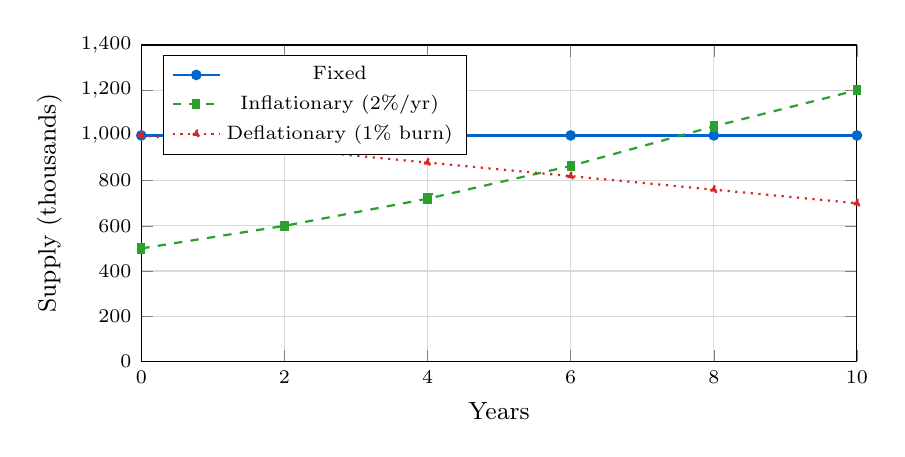
\begin{tikzpicture}
    \begin{axis}[
      width=0.88\textwidth, height=5.6cm,
      xlabel={Years}, ylabel={Supply (thousands)},
      xmin=0, xmax=10, ymin=0, ymax=1400,
      xtick={0,2,4,6,8,10},
      ytick={0,200,400,600,800,1000,1200,1400},
      grid=both, grid style={mlgray!30},
      legend pos=north west,
      legend style={font=\scriptsize},
      tick label style={font=\scriptsize},
      label style={font=\small},
    ]
      % Fixed supply
      \addplot[mlblue, solid, thick, mark=*, mark size=1.5pt]
        coordinates {(0,1000)(2,1000)(4,1000)(6,1000)(8,1000)(10,1000)};
      % Inflationary
      \addplot[mlgreen, dashed, thick, mark=square*, mark size=1.5pt]
        coordinates {(0,500)(2,600)(4,720)(6,865)(8,1040)(10,1200)};
      % Deflationary
      \addplot[mlred, dotted, thick, mark=triangle*, mark size=1.5pt]
        coordinates {(0,1000)(2,940)(4,880)(6,820)(8,760)(10,700)};
      \legend{Fixed, Inflationary (2\%/yr), Deflationary (1\% burn)}
    \end{axis}
  \end{tikzpicture}
  \end{center}
  \bottomnote{Token economics (tokenomics) significantly impacts long-term value and utility}
\end{frame}

% ----------------------------------------------------------
% Frame 43: Fixed Supply -- Digital Scarcity
% ----------------------------------------------------------
\begin{frame}{Fixed Supply -- Digital Scarcity}
  \begin{columns}[T]
    \column{0.45\textwidth}
      \begin{center}
      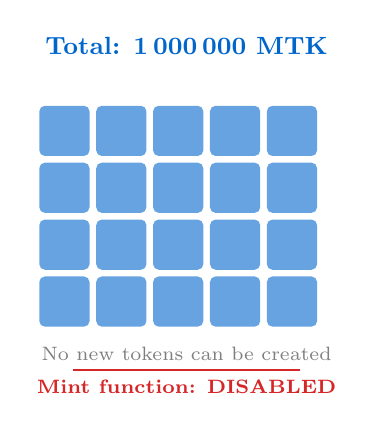
\begin{tikzpicture}[scale=0.85]
        % Title
        \node[font=\small\bfseries, mlblue] at (2.2, 4.2) {Total: 1\,000\,000 MTK};
        % Grid of filled blocks
        \foreach \x in {0,1,2,3,4} {
          \foreach \y in {0,1,2,3} {
            \fill[mlblue!60, rounded corners=2pt]
              (\x*0.85, \y*0.85) rectangle (\x*0.85+0.75, \y*0.85+0.75);
          }
        }
        % Lock symbol at bottom
        \node[font=\scriptsize, mlgray] at (2.2, -0.4) {No new tokens can be created};
        \draw[mlred, thick] (0.5, -0.65) -- (3.9, -0.65);
        \node[font=\scriptsize\bfseries, mlred] at (2.2, -0.9) {Mint function: DISABLED};
      \end{tikzpicture}
      \end{center}

    \column{0.52\textwidth}
      \begin{block}{\textcolor{mlgreen}{\checkmark} Pros}
        \begin{itemize}\setlength\itemsep{2pt}
          \item[\textcolor{mlgreen}{\textbullet}] Predictable scarcity
          \item[\textcolor{mlgreen}{\textbullet}] Deflationary price pressure
          \item[\textcolor{mlgreen}{\textbullet}] Simple to audit
        \end{itemize}
      \end{block}
      \begin{alertblock}{\textcolor{mlred}{\texttimes} Cons}
        \begin{itemize}\setlength\itemsep{2pt}
          \item[\textcolor{mlred}{\textbullet}] Cannot reward participants
          \item[\textcolor{mlred}{\textbullet}] No growth adaptation
          \item[\textcolor{mlred}{\textbullet}] Incentivizes hoarding
        \end{itemize}
      \end{alertblock}
      \smallskip
      {\scriptsize\textbf{Examples:} BTC (21M cap), similar model for MTK}
  \end{columns}
  \bottomnote{Fixed supply creates predictable scarcity -- but cannot adapt to ecosystem growth}
\end{frame}

% ----------------------------------------------------------
% Frame 44: Inflationary Models
% ----------------------------------------------------------
\begin{frame}{Inflationary Models}
  \begin{center}
  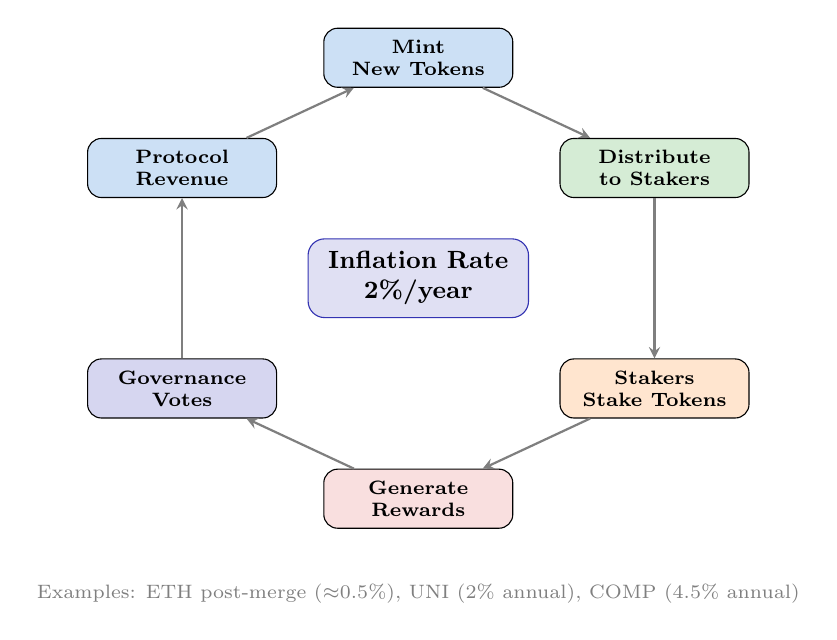
\begin{tikzpicture}[
    node distance=1.5cm,
    flowbox/.style={draw, rounded corners=5pt, minimum width=2.4cm,
                minimum height=0.75cm, font=\scriptsize\bfseries, align=center},
    arr/.style={->, >=stealth, thick, mlgray}
  ]
    % Center label
    \node[draw=mlpurple, rounded corners=6pt, fill=mlpurple!15,
          font=\small\bfseries, minimum width=2.8cm, minimum height=1.0cm,
          align=center] (center) at (0,0)
      {Inflation Rate\\2\%/year};

    % Surrounding nodes
    \node[flowbox, fill=mlblue!20]  (mint)    at (0, 2.8)   {Mint\\New Tokens};
    \node[flowbox, fill=mlgreen!20] (dist)    at (3.0, 1.4)  {Distribute\\to Stakers};
    \node[flowbox, fill=mlorange!20](stake)   at (3.0, -1.4) {Stakers\\Stake Tokens};
    \node[flowbox, fill=mlred!15]   (reward)  at (0, -2.8)  {Generate\\Rewards};
    \node[flowbox, fill=mlpurple!20](govern)  at (-3.0,-1.4) {Governance\\Votes};
    \node[flowbox, fill=mlblue!20]  (buyback) at (-3.0, 1.4) {Protocol\\Revenue};

    % Arrows around the cycle
    \draw[arr] (mint)    -- (dist);
    \draw[arr] (dist)    -- (stake);
    \draw[arr] (stake)   -- (reward);
    \draw[arr] (reward)  -- (govern);
    \draw[arr] (govern)  -- (buyback);
    \draw[arr] (buyback) -- (mint);

    % Examples
    \node[font=\scriptsize, mlgray, align=center] at (0, -4.0)
      {Examples: ETH post-merge ($\approx$0.5\%), UNI (2\% annual), COMP (4.5\% annual)};
  \end{tikzpicture}
  \end{center}
  \bottomnote{Inflationary models incentivize participation but must balance against dilution}
\end{frame}

% ----------------------------------------------------------
% Frame 45: Deflationary Models -- Burn Mechanics
% ----------------------------------------------------------
\begin{frame}{Deflationary Models -- Burn Mechanics}
  \begin{center}
  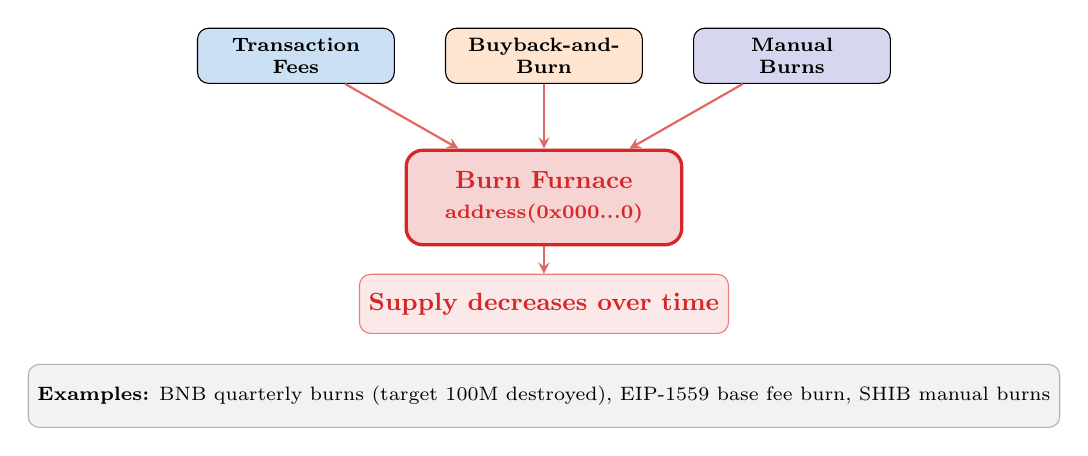
\begin{tikzpicture}[scale=0.9,
    srcbox/.style={draw, rounded corners=4pt, minimum width=2.5cm,
                minimum height=0.7cm, font=\scriptsize\bfseries, align=center},
    arr/.style={->, >=stealth, thick, mlred!70}
  ]
    % Source nodes
    \node[srcbox, fill=mlblue!20]   (fees)   at (-3.5, 3.2) {Transaction\\Fees};
    \node[srcbox, fill=mlorange!20] (buyb)   at (0, 3.2)    {Buyback-and-\\Burn};
    \node[srcbox, fill=mlpurple!20] (manual) at (3.5, 3.2)  {Manual\\Burns};

    % Burn furnace
    \node[draw=mlred, very thick, rounded corners=6pt, fill=mlred!20,
          minimum width=3.5cm, minimum height=1.2cm,
          font=\small\bfseries, align=center, text=mlred] (furnace) at (0, 1.2)
      {Burn Furnace\\{\scriptsize address(0x000...0)}};

    % Arrows into furnace
    \draw[arr] (fees)   -- (furnace);
    \draw[arr] (buyb)   -- (furnace);
    \draw[arr] (manual) -- (furnace);

    % Result
    \node[draw=mlred!60, rounded corners=4pt, fill=mlred!10,
          minimum width=4cm, minimum height=0.75cm,
          font=\small\bfseries, text=mlred, align=center] (result) at (0, -0.3)
      {Supply decreases over time};
    \draw[arr] (furnace) -- (result);

    % Examples box
    \node[draw=mlgray!60, rounded corners=4pt, fill=mlgray!10,
          minimum width=9cm, minimum height=0.8cm,
          font=\scriptsize, align=center] at (0, -1.6)
      {\textbf{Examples:} BNB quarterly burns (target 100M destroyed), EIP-1559 base fee burn,
       SHIB manual burns};
  \end{tikzpicture}
  \end{center}
  \bottomnote{Deflationary pressure increases scarcity -- but excessive burning can reduce liquidity}
\end{frame}

% ----------------------------------------------------------
% Frame 46: Distribution Strategies
% ----------------------------------------------------------
\begin{frame}{Distribution Strategies}
  \begin{columns}[T]
    \column{0.48\textwidth}
      \begin{center}
      {\small\bfseries Typical Allocation Ranges}\\[4pt]
      \begin{tabular}{@{}lc@{}}
        \toprule
        \textbf{Category} & \textbf{Typical Range} \\
        \midrule
        Team \& Founders   & 15--20\% \\
        Investors / VCs    & 10--20\% \\
        Public Sale        & 10--30\% \\
        Community/Airdrops & 10--20\% \\
        Ecosystem Fund     & 20--30\% \\
        Liquidity          &  5--15\% \\
        \bottomrule
      \end{tabular}
      \end{center}

    \column{0.50\textwidth}
      \begin{block}{\textcolor{mlgreen}{\checkmark} Best Practices}
        \begin{itemize}\setlength\itemsep{1pt}
          \scriptsize
          \item[\textcolor{mlgreen}{\checkmark}] Vesting schedules for insiders
          \item[\textcolor{mlgreen}{\checkmark}] Full on-chain transparency
          \item[\textcolor{mlgreen}{\checkmark}] Community-first allocation
          \item[\textcolor{mlgreen}{\checkmark}] Gradual release schedules
        \end{itemize}
      \end{block}
      \begin{alertblock}{\textcolor{mlred}{\texttimes} Red Flags}
        \begin{itemize}\setlength\itemsep{1pt}
          \scriptsize
          \item[\textcolor{mlred}{\texttimes}] $>$50\% allocated to team
          \item[\textcolor{mlred}{\texttimes}] No vesting for founders
          \item[\textcolor{mlred}{\texttimes}] Hidden allocations
          \item[\textcolor{mlred}{\texttimes}] Instant unlock at launch
        \end{itemize}
      \end{alertblock}
  \end{columns}
  \bottomnote{Transparent tokenomics build trust -- always publish distribution details}
\end{frame}

% ----------------------------------------------------------
% Frame 47: Distribution Visualization (Manual TikZ pie chart)
% ----------------------------------------------------------
\begin{frame}{Distribution Visualization}
  \begin{center}
  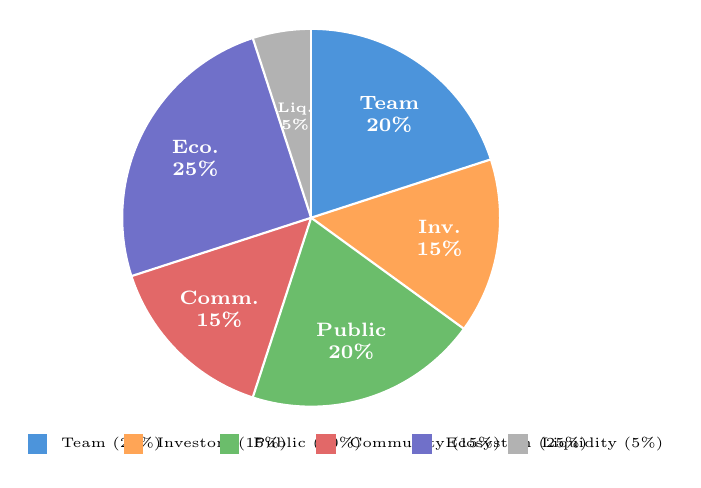
\begin{tikzpicture}[scale=1.0]
    % Pie chart using manual \fill arcs
    % Slices: Team 20%, Investors 15%, Public 20%, Community 15%, Ecosystem 25%, Liquidity 5%
    % Degrees: 72, 54, 72, 54, 90, 18
    % Cumulative start angles: 90, 18, -36, -108, -162, -252 (going clockwise from top)
    \def\r{2.4}

    % Team 20% (mlblue!70): 90 to 18
    \fill[mlblue!70]  (0,0) -- (\r*0.0, \r*1.0)
      arc[start angle=90, end angle=18, radius=\r] -- cycle;

    % Investors 15% (mlorange!70): 18 to -36
    \fill[mlorange!70] (0,0) -- (\r*0.951, \r*0.309)
      arc[start angle=18, end angle=-36, radius=\r] -- cycle;

    % Public Sale 20% (mlgreen!70): -36 to -108
    \fill[mlgreen!70] (0,0) -- (\r*0.809, \r*-0.588)
      arc[start angle=-36, end angle=-108, radius=\r] -- cycle;

    % Community 15% (mlred!70): -108 to -162
    \fill[mlred!70]  (0,0) -- (\r*-0.309, \r*-0.951)
      arc[start angle=-108, end angle=-162, radius=\r] -- cycle;

    % Ecosystem 25% (mlpurple!70): -162 to -252
    \fill[mlpurple!70] (0,0) -- (\r*-0.951, \r*-0.309)
      arc[start angle=-162, end angle=-252, radius=\r] -- cycle;

    % Liquidity 5% (mlgray!70): -252 to -270
    \fill[mlgray!60] (0,0) -- (\r*-0.309, \r*0.951)
      arc[start angle=-252, end angle=-270, radius=\r] -- cycle;

    % Slice outlines
    \draw[white, thick] (0,0) circle (\r);
    \draw[white, thick] (0,0) -- (0, \r);
    \draw[white, thick] (0,0) -- (\r*0.951, \r*0.309);
    \draw[white, thick] (0,0) -- (\r*0.809, \r*-0.588);
    \draw[white, thick] (0,0) -- (\r*-0.309, \r*-0.951);
    \draw[white, thick] (0,0) -- (\r*-0.951, \r*-0.309);
    \draw[white, thick] (0,0) -- (\r*-0.309, \r*0.951);

    % Labels (placed at midpoint of each slice)
    \node[font=\scriptsize\bfseries, white, align=center] at (53:1.65) {Team\\20\%};
    \node[font=\scriptsize\bfseries, white, align=center] at (-9:1.65)  {Inv.\\15\%};
    \node[font=\scriptsize\bfseries, white, align=center] at (-72:1.65) {Public\\20\%};
    \node[font=\scriptsize\bfseries, white, align=center] at (-135:1.65){Comm.\\15\%};
    \node[font=\scriptsize\bfseries, white, align=center] at (-207:1.65){Eco.\\25\%};
    \node[font=\tiny\bfseries, white, align=center]       at (-261:1.3) {Liq.\\5\%};

    % Legend row below
    \fill[mlblue!70] (-3.6, -3.0) rectangle (-3.35, -2.75);
    \node[font=\tiny, anchor=west] at (-3.3, -2.875) {Team (20\%)};
    \fill[mlorange!70] (-2.38, -3.0) rectangle (-2.13, -2.75);
    \node[font=\tiny, anchor=west] at (-2.08, -2.875) {Investors (15\%)};
    \fill[mlgreen!70] (-1.16, -3.0) rectangle (-0.91, -2.75);
    \node[font=\tiny, anchor=west] at (-0.86, -2.875) {Public (20\%)};
    \fill[mlred!70] (0.06, -3.0) rectangle (0.31, -2.75);
    \node[font=\tiny, anchor=west] at (0.36, -2.875) {Community (15\%)};
    \fill[mlpurple!70] (1.28, -3.0) rectangle (1.53, -2.75);
    \node[font=\tiny, anchor=west] at (1.58, -2.875) {Ecosystem (25\%)};
    \fill[mlgray!60] (2.50, -3.0) rectangle (2.75, -2.75);
    \node[font=\tiny, anchor=west] at (2.80, -2.875) {Liquidity (5\%)};
  \end{tikzpicture}
  \end{center}
  \bottomnote{Distribution determines initial decentralization and long-term governance power}
\end{frame}

% ----------------------------------------------------------
% Frame 48: Vesting Schedules
% ----------------------------------------------------------
\begin{frame}{Vesting Schedules}
  \begin{center}
  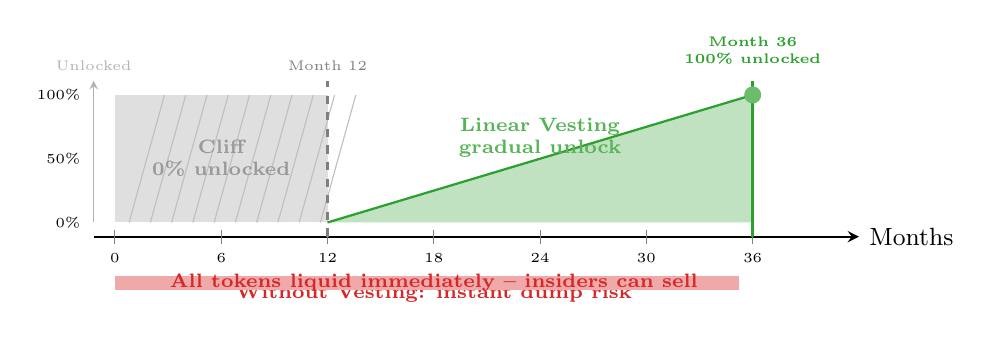
\begin{tikzpicture}[scale=0.9]
    % Timeline axis
    \draw[->, >=stealth, thick] (-0.3, 0) -- (10.5, 0) node[right, font=\small] {Months};
    \foreach \m/\x in {0/0, 6/1.5, 12/3, 18/4.5, 24/6, 30/7.5, 36/9} {
      \draw[mlgray] (\x, -0.1) -- (\x, 0.1);
      \node[font=\tiny, below] at (\x, -0.1) {\m};
    }

    % Cliff period (0-12 months): hatched gray
    \fill[mlgray!25] (0, 0.2) rectangle (3, 2.0);
    \foreach \xx in {0.2,0.5,0.8,1.1,1.4,1.7,2.0,2.3,2.6,2.9} {
      \draw[mlgray!50, thin] (\xx, 0.2) -- (\xx+0.5, 2.0);
    }
    \node[font=\scriptsize\bfseries, align=center, mlgray!80] at (1.5, 1.1)
      {Cliff\\0\% unlocked};
    \draw[mlgray, thick, dashed] (3, 0) -- (3, 2.2);
    \node[font=\tiny, mlgray, above] at (3, 2.2) {Month 12};

    % Linear vesting (12-36 months): gradient green fill
    \fill[mlgreen!30] (3, 0.2) -- (9, 0.2) -- (9, 2.0) -- (3, 0.2) -- cycle;
    \draw[mlgreen, thick] (3, 0.2) -- (9, 2.0);
    \node[font=\scriptsize\bfseries, align=center, mlgreen!80] at (6, 1.4)
      {Linear Vesting\\gradual unlock};

    % Full unlock marker at 36 months
    \draw[mlgreen, very thick] (9, 0) -- (9, 2.2);
    \fill[mlgreen!70] (9, 2.0) circle (0.12);
    \node[font=\tiny\bfseries, mlgreen, above, align=center] at (9, 2.3)
      {Month 36\\100\% unlocked};

    % Unlock percentage axis
    \draw[->, >=stealth, mlgray!60] (-0.3, 0.2) -- (-0.3, 2.2)
      node[above, font=\tiny] {Unlocked};
    \foreach \pct/\y in {0/0.2, 50/1.1, 100/2.0} {
      \node[font=\tiny, left] at (-0.35, \y) {\pct\%};
    }

    % Without Vesting warning below
    \node[font=\scriptsize\bfseries, mlred] at (4.5, -0.8)
      {Without Vesting: instant dump risk};
    \draw[->, >=stealth, mlred, thick] (0.3, -0.65) -- (8.5, -0.65);
    \fill[mlred!40] (0.0, -0.75) rectangle (8.8, -0.55);
    \node[font=\scriptsize\bfseries, mlred] at (4.5, -0.65)
      {All tokens liquid immediately -- insiders can sell};
  \end{tikzpicture}
  \end{center}
  \bottomnote{Vesting protects investors by preventing large token dumps after launch}
\end{frame}

% ----------------------------------------------------------
% Frame 49: Real-World Token Economics
% ----------------------------------------------------------
\begin{frame}{Real-World Token Economics}
  \begin{center}
  {\small
  \begin{tabular}{@{}llllp{2.5cm}@{}}
    \toprule
    \textbf{Token} & \textbf{Type} & \textbf{Supply Model} & \textbf{Max Supply} & \textbf{Primary Use} \\
    \midrule
    USDC  & Stablecoin  & Elastic (mint/redeem)     & Unlimited & Payments \\
    LINK  & Utility     & Fixed                     & 1B        & Oracle payments \\
    UNI   & Governance  & Inflationary (2\%)        & 1B initial& Protocol governance \\
    AAVE  & DeFi        & Deflationary (buyback)    & 16M       & Lending governance \\
    BNB   & Exchange    & Deflationary (burns)      & 200M      & Fee discounts \\
    MATIC & L2          & Fixed                     & 10B       & Gas token \\
    \bottomrule
  \end{tabular}
  }
  \end{center}
  \bottomnote{Study successful tokens to understand what makes sustainable token economics}
\end{frame}

% ----------------------------------------------------------
% Frame 50: [CODE] Tokenomics in Code  -- FRAGILE required
% ----------------------------------------------------------
\begin{frame}[fragile]{Tokenomics in Code}
  \begin{columns}[T]
    \column{0.32\textwidth}
      \begin{block}{\scriptsize Fixed Supply}
        \begin{lstlisting}[basicstyle=\tiny\ttfamily,
            language=Solidity,
            breaklines=true]
// Fixed: mint all at deploy
constructor()
  ERC20("Fixed","FIX")
{
  _mint(msg.sender,
    1e6 * 1e18);
}
// No mint() exists
        \end{lstlisting}
      \end{block}

    \column{0.32\textwidth}
      \begin{block}{\scriptsize Inflationary}
        \begin{lstlisting}[basicstyle=\tiny\ttfamily,
            language=Solidity,
            breaklines=true]
// Owner can mint more
function mint(
    address to,
    uint256 amt
) public onlyOwner {
  _mint(to, amt);
}
        \end{lstlisting}
      \end{block}

    \column{0.34\textwidth}
      \begin{block}{\scriptsize Deflationary}
        \begin{lstlisting}[basicstyle=\tiny\ttfamily,
            language=Solidity,
            breaklines=true]
// 1% burn on transfer
function transfer(
    address to, uint amt
) public override
  returns (bool) {
  uint fee = amt / 100;
  _burn(msg.sender, fee);
  return super.transfer(
    to, amt - fee);
}
        \end{lstlisting}
      \end{block}
  \end{columns}
  \bottomnote{Supply model choice is encoded permanently in the smart contract -- choose wisely}
\end{frame}

% ----------------------------------------------------------
% Frame 51: Token Valuation Frameworks
% ----------------------------------------------------------
\begin{frame}{Token Valuation Frameworks}
  \begin{center}
  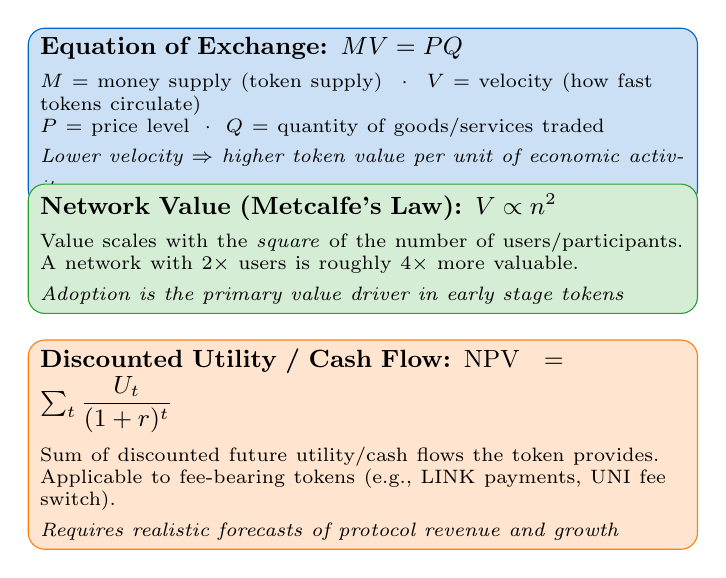
\begin{tikzpicture}[scale=0.9,
    fbox/.style={rounded corners=6pt,
                 minimum width=8.5cm, minimum height=1.6cm,
                 text width=8.2cm, align=left, font=\small}
  ]
    % Box 1: Equation of Exchange
    \node[fbox, draw=mlblue, fill=mlblue!20, anchor=north] (eq) at (0, 4.0) {%
      \textbf{Equation of Exchange:} $MV = PQ$\\[4pt]
      \scriptsize $M$ = money supply (token supply)
      $\;\cdot\;$ $V$ = velocity (how fast tokens circulate)\\
      $P$ = price level $\;\cdot\;$ $Q$ = quantity of goods/services traded\\
      \textit{Lower velocity $\Rightarrow$ higher token value per unit of economic activity}
    };

    % Box 2: Network Value
    \node[fbox, draw=mlgreen, fill=mlgreen!20, anchor=north] (nv) at (0, 1.8) {%
      \textbf{Network Value (Metcalfe's Law):} $V \propto n^{2}$\\[4pt]
      \scriptsize Value scales with the \emph{square} of the number of users/participants.\\
      A network with $2\times$ users is roughly $4\times$ more valuable.\\
      \textit{Adoption is the primary value driver in early stage tokens}
    };

    % Box 3: Discounted Utility
    \node[fbox, draw=mlorange, fill=mlorange!20, anchor=north] (du) at (0, -0.4) {%
      \textbf{Discounted Utility / Cash Flow:} $\mathrm{NPV} = \sum_t \dfrac{U_t}{(1+r)^t}$\\[4pt]
      \scriptsize Sum of discounted future utility/cash flows the token provides.\\
      Applicable to fee-bearing tokens (e.g., LINK payments, UNI fee switch).\\
      \textit{Requires realistic forecasts of protocol revenue and growth}
    };
  \end{tikzpicture}
  \end{center}
  \bottomnote{Token valuation is an emerging field -- no single framework captures all value drivers}
\end{frame}

% ===========================================================
\section{Advanced Topics \& Summary}
% ===========================================================

% ----------------------------------------------------------
% Frame 52: Section Divider
% ----------------------------------------------------------
\begin{frame}[plain]
  \begin{beamercolorbox}[wd=\paperwidth, ht=\paperheight, center, sep=0pt]{mlpurple}
    \vfill
    {\color{white}\LARGE Section 5: Advanced Topics \& Summary}\\[1em]
    {\color{white!80}\large Next steps and key takeaways}
    \vfill
  \end{beamercolorbox}
\end{frame}

% ----------------------------------------------------------
% Frame 53: Deployment Pipeline
% ----------------------------------------------------------
\begin{frame}{Deployment Pipeline}
  \begin{center}
  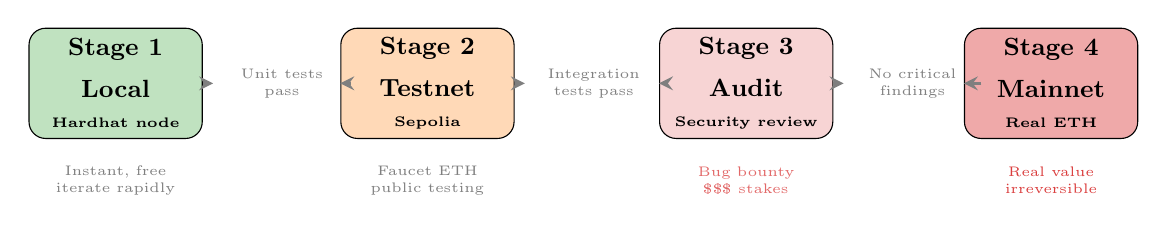
\begin{tikzpicture}[scale=0.88,
    stage/.style={draw, rounded corners=6pt,
                  minimum width=2.2cm, minimum height=1.4cm,
                  font=\small\bfseries, align=center},
    gate/.style={font=\tiny, mlgray, align=center, text width=1.5cm},
    arr/.style={->, >=stealth, very thick, mlgray}
  ]
    % Stage 1: Local
    \node[stage, fill=mlgreen!30] (local) at (0, 0)
      {Stage 1\\[4pt]Local\\{\tiny Hardhat node}};

    % Gate 1->2
    \node[gate] (g1) at (2.4, 0)
      {Unit tests\\pass};
    \draw[arr] (local) -- (g1);

    % Stage 2: Testnet
    \node[stage, fill=mlorange!30] (testnet) at (4.5, 0)
      {Stage 2\\[4pt]Testnet\\{\tiny Sepolia}};
    \draw[arr] (g1) -- (testnet);

    % Gate 2->3
    \node[gate] (g2) at (6.9, 0)
      {Integration\\tests pass};
    \draw[arr] (testnet) -- (g2);

    % Stage 3: Audit
    \node[stage, fill=mlred!20] (audit) at (9.1, 0)
      {Stage 3\\[4pt]Audit\\{\tiny Security review}};
    \draw[arr] (g2) -- (audit);

    % Gate 3->4
    \node[gate] (g3) at (11.5, 0)
      {No critical\\findings};
    \draw[arr] (audit) -- (g3);

    % Stage 4: Mainnet
    \node[stage, fill=mlred!40] (mainnet) at (13.5, 0)
      {Stage 4\\[4pt]Mainnet\\{\tiny Real ETH}};
    \draw[arr] (g3) -- (mainnet);

    % Annotations below each stage
    \node[font=\tiny, mlgray, align=center, text width=2cm] at (0, -1.4)
      {Instant, free\\iterate rapidly};
    \node[font=\tiny, mlgray, align=center, text width=2cm] at (4.5, -1.4)
      {Faucet ETH\\public testing};
    \node[font=\tiny, mlred!70, align=center, text width=2cm] at (9.1, -1.4)
      {Bug bounty\\\$\$\$ stakes};
    \node[font=\tiny, mlred!90, align=center, text width=2.0cm] at (13.5, -1.4)
      {Real value\\irreversible};
  \end{tikzpicture}
  \end{center}
  \bottomnote{Each stage adds risk -- never skip testing stages}
\end{frame}

% ----------------------------------------------------------
% Frame 54: Testnet Deployment
% ----------------------------------------------------------
\begin{frame}{Testnet Deployment}
  \begin{columns}[T]
    \column{0.46\textwidth}
      \begin{center}
      {\small\bfseries Available Testnets}\\[4pt]
      \begin{tabular}{@{}lll@{}}
        \toprule
        \textbf{Network} & \textbf{Faucet} & \textbf{Block Time} \\
        \midrule
        Sepolia   & sepolia-faucet.com   & 12s \\
        Goerli    & goerlifaucet.com     & 12s \\
        Mumbai    & faucet.polygon.tech  & 2s  \\
        \bottomrule
      \end{tabular}
      \end{center}

    \column{0.52\textwidth}
      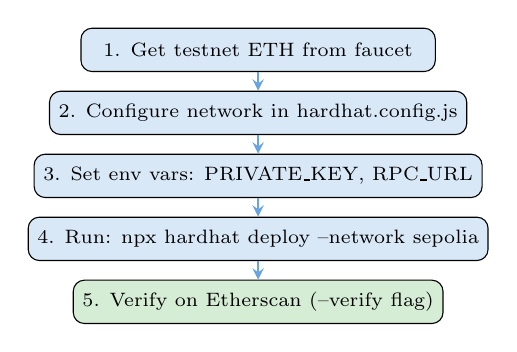
\begin{tikzpicture}[
        stepbox/.style={draw, rounded corners=4pt, fill=mlblue!15,
                     minimum width=4.5cm, minimum height=0.55cm,
                     font=\scriptsize, align=center},
        arr/.style={->, >=stealth, thick, mlblue!60}
      ]
        \node[stepbox] (s1) at (0, 4.0) {1. Get testnet ETH from faucet};
        \node[stepbox] (s2) at (0, 3.2) {2. Configure network in hardhat.config.js};
        \node[stepbox] (s3) at (0, 2.4) {3. Set env vars: PRIVATE\_KEY, RPC\_URL};
        \node[stepbox] (s4) at (0, 1.6) {4. Run: npx hardhat deploy --network sepolia};
        \node[stepbox, fill=mlgreen!20] (s5) at (0, 0.8)
          {5. Verify on Etherscan (--verify flag)};
        \draw[arr] (s1)--(s2); \draw[arr] (s2)--(s3);
        \draw[arr] (s3)--(s4); \draw[arr] (s4)--(s5);
      \end{tikzpicture}
  \end{columns}
  \bottomnote{Testnet deployment is essential practice -- treat it like production}
\end{frame}

% ----------------------------------------------------------
% Frame 55: Security Considerations
% ----------------------------------------------------------
\begin{frame}{Security Considerations}
  \begin{columns}[T]
    \column{0.48\textwidth}
      \begin{alertblock}{Common Vulnerabilities}
        \begin{itemize}\setlength\itemsep{2pt}
          \scriptsize
          \item[\textcolor{mlred}{\textbullet}] Reentrancy attacks
          \item[\textcolor{mlred}{\textbullet}] Integer overflow/underflow
          \item[\textcolor{mlred}{\textbullet}] Access control flaws
          \item[\textcolor{mlred}{\textbullet}] Front-running attacks
          \item[\textcolor{mlred}{\textbullet}] Approval race condition (ERC-20)
          \item[\textcolor{mlred}{\textbullet}] Centralized admin keys
        \end{itemize}
      \end{alertblock}

    \column{0.50\textwidth}
      \begin{block}{Best Practices}
        \begin{itemize}\setlength\itemsep{2pt}
          \scriptsize
          \item[\textcolor{mlgreen}{\checkmark}] Use OpenZeppelin battle-tested contracts
          \item[\textcolor{mlgreen}{\checkmark}] Checks-Effects-Interactions pattern
          \item[\textcolor{mlgreen}{\checkmark}] Add \texttt{ReentrancyGuard} modifier
          \item[\textcolor{mlgreen}{\checkmark}] Implement \texttt{Pausable} pattern
          \item[\textcolor{mlgreen}{\checkmark}] Multi-sig for admin ownership
          \item[\textcolor{mlgreen}{\checkmark}] External audit before mainnet
        \end{itemize}
      \end{block}
  \end{columns}
  \bottomnote{Smart contract bugs are permanent and can result in total loss of funds}
\end{frame}

% ----------------------------------------------------------
% Frame 56: Security Tools
% ----------------------------------------------------------
\begin{frame}{Security Tools}
  \begin{center}
  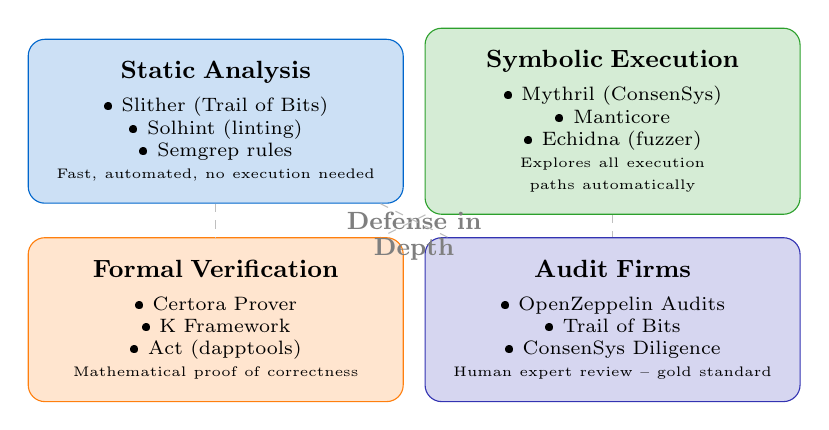
\begin{tikzpicture}[scale=0.9,
    cat/.style={rounded corners=6pt,
                minimum width=4.5cm, text width=4.2cm,
                font=\scriptsize, align=center, inner sep=8pt}
  ]
    % Category 1: Static Analysis
    \node[cat, draw=mlblue, fill=mlblue!20] (sa) at (-2.8, 1.6) {%
      \textbf{\small Static Analysis}\\[4pt]
      \textbullet\ Slither (Trail of Bits)\\
      \textbullet\ Solhint (linting)\\
      \textbullet\ Semgrep rules\\
      {\tiny Fast, automated, no execution needed}
    };

    % Category 2: Symbolic Execution
    \node[cat, draw=mlgreen, fill=mlgreen!20] (sym) at (2.8, 1.6) {%
      \textbf{\small Symbolic Execution}\\[4pt]
      \textbullet\ Mythril (ConsenSys)\\
      \textbullet\ Manticore\\
      \textbullet\ Echidna (fuzzer)\\
      {\tiny Explores all execution paths automatically}
    };

    % Category 3: Formal Verification
    \node[cat, draw=mlorange, fill=mlorange!20] (fv) at (-2.8, -1.2) {%
      \textbf{\small Formal Verification}\\[4pt]
      \textbullet\ Certora Prover\\
      \textbullet\ K Framework\\
      \textbullet\ Act (dapptools)\\
      {\tiny Mathematical proof of correctness}
    };

    % Category 4: Audit Firms
    \node[cat, draw=mlpurple, fill=mlpurple!20] (af) at (2.8, -1.2) {%
      \textbf{\small Audit Firms}\\[4pt]
      \textbullet\ OpenZeppelin Audits\\
      \textbullet\ Trail of Bits\\
      \textbullet\ ConsenSys Diligence\\
      {\tiny Human expert review -- gold standard}
    };

    % Center connector
    \node[font=\small\bfseries, mlgray] at (0, 0.2)
      {Defense in};
    \node[font=\small\bfseries, mlgray] at (0, -0.2)
      {Depth};
    \draw[mlgray!50, dashed] (sa) -- (fv);
    \draw[mlgray!50, dashed] (sym) -- (af);
    \draw[mlgray!50, dashed] (sa) -- (af);
    \draw[mlgray!50, dashed] (sym) -- (fv);
  \end{tikzpicture}
  \end{center}
  \bottomnote{Use multiple security tools -- no single tool catches everything}
\end{frame}

% ----------------------------------------------------------
% Frame 57: Final Project Overview
% ----------------------------------------------------------
\begin{frame}{Final Project Overview}
  \begin{columns}[T]
    \column{0.48\textwidth}
      \begin{block}{Deliverables}
        \begin{itemize}\setlength\itemsep{4pt}
          \item[\textcolor{mlblue}{\textbullet}]
            \textbf{Custom ERC-20 token} with chosen supply model and extensions
          \item[\textcolor{mlblue}{\textbullet}]
            \textbf{Comprehensive test suite} (\(\geq\)90\% coverage, Hardhat)
          \item[\textcolor{mlblue}{\textbullet}]
            \textbf{Testnet deployment} with verified Etherscan contract
          \item[\textcolor{mlblue}{\textbullet}]
            \textbf{README documentation} with tokenomics rationale
        \end{itemize}
      \end{block}

    \column{0.50\textwidth}
      \begin{block}{Evaluation Criteria}
        \begin{itemize}\setlength\itemsep{3pt}
          \scriptsize
          \item[\textcolor{mlblue}{\textbullet}]
            \textbf{Code quality} (readability, comments, style) \hfill \textbf{30\%}
          \item[\textcolor{mlgreen}{\textbullet}]
            \textbf{Test coverage} (breadth, edge cases) \hfill \textbf{25\%}
          \item[\textcolor{mlred}{\textbullet}]
            \textbf{Security} (no known vulnerabilities) \hfill \textbf{25\%}
          \item[\textcolor{mlorange}{\textbullet}]
            \textbf{Creativity} (unique features, tokenomics) \hfill \textbf{20\%}
        \end{itemize}
      \end{block}
  \end{columns}
  \bottomnote{This project integrates all 4 lessons: blockchain, cryptography, smart contracts, and tokens}
\end{frame}

% ----------------------------------------------------------
% Frame 58: Key Takeaways
% ----------------------------------------------------------
\begin{frame}{Key Takeaways}
  \begin{center}
  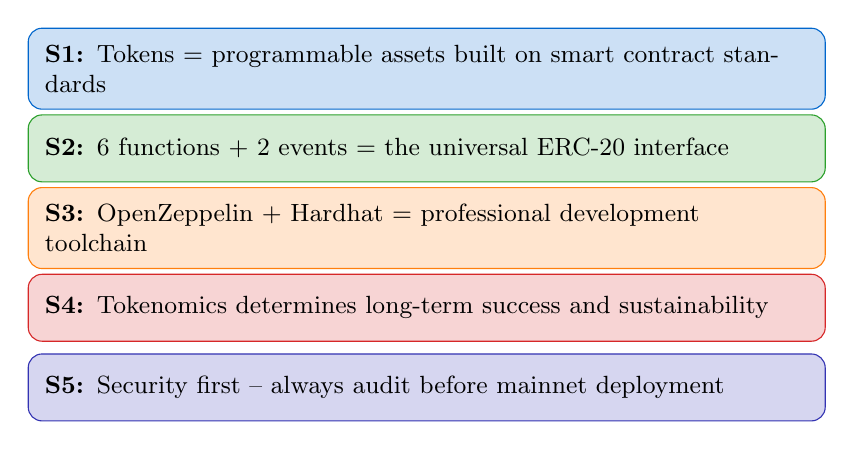
\begin{tikzpicture}[scale=0.92,
    tkbox/.style={rounded corners=5pt,
                minimum width=10cm, minimum height=0.85cm,
                text width=9.7cm, font=\small, align=left, inner sep=6pt}
  ]
    \node[tkbox, draw=mlblue, fill=mlblue!20]    at (0, 3.4)
      {\textbf{S1:} Tokens = programmable assets built on smart contract standards};
    \node[tkbox, draw=mlgreen, fill=mlgreen!20]   at (0, 2.3)
      {\textbf{S2:} 6 functions + 2 events = the universal ERC-20 interface};
    \node[tkbox, draw=mlorange, fill=mlorange!20]  at (0, 1.2)
      {\textbf{S3:} OpenZeppelin + Hardhat = professional development toolchain};
    \node[tkbox, draw=mlred, fill=mlred!20]     at (0, 0.1)
      {\textbf{S4:} Tokenomics determines long-term success and sustainability};
    \node[tkbox, draw=mlpurple, fill=mlpurple!20]  at (0, -1.0)
      {\textbf{S5:} Security first -- always audit before mainnet deployment};
  \end{tikzpicture}
  \end{center}
  \bottomnote{You now have the foundation to build, deploy, and evaluate ERC-20 tokens}
\end{frame}

% ----------------------------------------------------------
% Frame 59: Course Completion
% ----------------------------------------------------------
\begin{frame}{Course Completion}
  \begin{columns}[T]
    \column{0.44\textwidth}
      \begin{center}
      {\small\bfseries Course Overview}\\[4pt]
      \begin{tabular}{@{}ll@{}}
        \toprule
        \textbf{Lesson} & \textbf{Topic} \\
        \midrule
        L01 & Blockchain Fundamentals \\
        L02 & Cryptography \\
        L03 & Smart Contracts \\
        L04 & Token Creation \\
        \bottomrule
      \end{tabular}
      \end{center}

    \column{0.54\textwidth}
      \begin{block}{You Can Now}
        \begin{itemize}\setlength\itemsep{1pt}
          \scriptsize
          \item[\textcolor{mlgreen}{\checkmark}] Write ERC-20 token contracts
          \item[\textcolor{mlgreen}{\checkmark}] Deploy to testnets \& mainnet
          \item[\textcolor{mlgreen}{\checkmark}] Evaluate tokenomics models
          \item[\textcolor{mlgreen}{\checkmark}] Assess smart contract security
        \end{itemize}
      \end{block}
      \begin{block}{Continue Learning}
        \begin{itemize}\setlength\itemsep{1pt}
          \scriptsize
          \item[\(\rightarrow\)] NFTs (ERC-721, ERC-1155)
          \item[\(\rightarrow\)] DeFi protocols (Uniswap, Aave)
          \item[\(\rightarrow\)] DAOs and governance
          \item[\(\rightarrow\)] L2 scaling (Rollups, Polygon)
          \item[\(\rightarrow\)] Security auditing
        \end{itemize}
      \end{block}
  \end{columns}
  \bottomnote{The blockchain space evolves rapidly -- continuous learning is essential}
\end{frame}

\end{document}

